\chapter{Introduction to GUI}
\label{chap:introduction}

A graphics library is a library with API dealing with graphics.
A widget toolkit is a particular type of graphics library with APIs supporting
the look-and-feel of different graphical components in a window such as text
box, menu, \ldots The GUI development refers to the use of a proper widget
toolkits. However, these different widget toolkits need to use a particular
graphics library.

We will first cover the history of graphics library in different platform, and 
the different widget toolkits accordingly.

Today, the general attitude is that the GUI should be Web-based. It means that
we are transforming from Desktop-based applications to Web-based applications.
\begin{enumerate}
  \item ASP.NET MVC version 4+
\end{enumerate}

\section{Windows Managers vs Login Managers Vs Display
Managers Vs Desktop Environment vs Windowing System}

First, remember the booting order (See Sys-admin book - Sect.\ref{sec:booting}).

Remember that when you start a session (locally or remotely) on Windows or
Linux, a session needs to be created to a windowing system.
 
\begin{itemize}
 \item create a session: either a console session (e.g. via SSH), or an
 X-session (e.g. via locally run machine as launched by the display manager
 (Sect.\ref{sec:Display_manager})) In the case X11 is the windowing system, we have an
 X-session (Sect.\ref{sec:X-session}).

  \item an session to the windowing system, e.g. X Session 
  
  
  
  \item a login screen: as defined by a Login Manager (what to show on that
  screen, and any visual effect as well as background)
  
  
  \item 
\end{itemize}

  A windowing system (Display Server) is a component of the desktop environment
  (Sect.\ref{sec:desktop_environment}) which supports the implementation of a
  window manager (Sect.\ref{sec:window_manager}). 
  From the programmer's point of views, a windowing system implements graphical
  primitives, e.g. rendering fonts or drawing a ling on the screen.  
  Most windowing systems implements WIMP (windows, icons,
  menus and pointer) paradigm for a UI. Example: X11 (X Window System),
  Wayland (Sect.\ref{sec:Wayland}), Xorg (Sect.\ref{sec:Xorg}), XFree86
  (Sect.\ref{sec:XFree86}), Mir (Sect.\ref{sec:Mir}).
%    A display server create the graphical environment: Example: Xorg,
%   XFree86, X11, Mir, Wayland. 
%   
   
  Most windowing systems have basic support of re-parenting which allows windows
  to overlap, however the ways in which windows interact is usually controlled
  by the window manager. Some windowing systems, e.g. X11, allow user to display
  the graphical applications running on a remote machine. 
  
  A windowing system does not define the 'look and feel', it just
  control the interactions between windows or components. The 'looks and feel'
  is defined by the window manager, widget toolkit, and desktop environment.
  A typical desktop environemnt consists of several separate components: 
\begin{enumerate}
% It needs to use a window manager
%   (Sect.\ref{sec:window_manager})
%   
%   
  
  \item A window manager (Sect.\ref{sec:window_manager}): control the placement
  and decoration of windows, i.e. window border and controls. Some window
  manager are the stand-alone, e.g. WindowMaker, sawfish, fvwm, Metacity,
  Mutter \ldots Some depend on an accompanying desktop environment.
  
  NOTE: Some window managers (e.g. WindowMaker, ROX Desktop) integrates other
  desktop environment elements, e.g. integrated file manager.
  
  \item A display manager (i.e. a login manager): the first X program run by the
  system if the system is starting X and allows you to log on to the local
  system, or network system. Example: [gkx]dm
  
  \item file manager (e.g. Nautilus, Dolphin)
  
  \item a set of graphical themes
  
  \item widget tookits:   A widget tookit is required to draw the WIMP, e.g.  GTK+, Clutter, Qt.
   
  \item other libraries: for managing the desktop
\end{enumerate}

A desktop environment (): a suite of applications designed to integrate well
with each other to provide a consistent experience, e.g. XFCE, KDE, GNOME.

For Web, there are also Web windowing systems, e.g. Dojo, ExtJS, Web Window
Manager. 
  
Some operating system, e.g. MS Windows, Mac OS, has its windowing system
integrated with the O/S. Windows 7/8 use Aero windowing environment.
   
\section{History of 2D graphics library in Linux}
\label{sec:2D-graphics-Linux}

\subsection{X Windows system: X server, X client}
\label{sec:X-protocol}
\label{sec:X-system}
\label{sec:display-server}

To provide a basic framework for GUI environment that allows any GUI
applications to work with the graphics hardware, a protocol known as X or {\bf X
Window System} was developed (from MIT in 1984).
This is also a {\it network protocol} as the application can run on one machine
and its GUI is displayed on a different machine.
{\bf X Window System} has a stable and generic APIs that deal with how a GUI
component (e.g. windows) is (1) drawn or moved on the display device, and (2)
interacted with the mouse and keyboard (and recently touchscreen), independent
from the underlying hardware device.

In the early times, X server was only the single piece of software that had
direct access to the graphics hardware.
So, the GUI applications would do all their drawing indirectly, through the X
server. Sect.\ref{sec:X-client-implementation} discusses how a GUI application
interact with the X server.

The  {\bf network protocol} is a client-server model. So, we needs two
implementation. 
\begin{enumerate}
\item {\bf X clients} are GUI programs (web browser, xterm, ...)

\item {\bf X server} (e.g. X.org implementation): a program that manage the
interaction between X clients and hardware (mouse, keyboard, display)
\end{enumerate}
% It means that it allows user to run the {\it client} program on
% a remote machine, and the user interface is displayed on the local machine (known as
% \textcolor{red}{display server} or {\bf X server}).

The machine on which the GUI of the application is displayed run {\bf X server},
and the machine that actually hosts the application (i.e. it handles the
processing the data) has {\bf X client}, and whatever is supposed to be display
on the GUI will be sent to the X server for rendering the GUI of the
application. If the two machines are one, X server and X
client run on the same machine.


\subsection{-- X11 (XWindow)}
\label{sec:X11}

The most recent major version of X system (Sect.\ref{sec:X-protocol}) is 11,
known as X11 (or X Windows system at the current major version 11). X11 has gone
through Release 3, Release 4, Release 5, Release 6 (X11R6) and Release 7
(X11R7). X Server version 11 Release 1, aka X11R1, was released in Sep-1987.
This is the most widely used version, so X Window System is often called {\bf
X11}. Nowaday, a competing implementation is Wayland protocol
(Sect.\ref{sec:Wayland}). Each new extension to the X11 protocol adds requests
that clients can make to the X server. 

X11R7 includes
\begin{minipage}[t]{0.5\textwidth}
\begin{verbatim}
X11R7.0
X11R7.1
X11R7.2
X11R7.3
X11R7.4
\end{verbatim}
\end{minipage}
\begin{minipage}[t]{0.5\textwidth}
\begin{verbatim}
X11R7.5
X11R7.6-RC1
X11R7.6
X11R7.7-RC1
X11R7.7
\end{verbatim}
\end{minipage}

Nowadays, {\bf X11} is built as an abstraction layer on top of the operating
system kernel to provide basic GUI for networked computers. The different implementation of 
\begin{itemize}
  \item X server is discussed in Sect.\ref{sec:X-server-implementation}.
  \item X client is discussed in Sect.\ref{sec:X-client-implementation}.
\end{itemize}

In order to understand X11, we need to know about XFree86
(Sect.\ref{sec:XFree86}, as both are closely related.  XFree86 is the most
common variant running on Unix-like systems until 2004, then being taken over by
{\bf X.org Foundation} -  many team members from XFree86 joined X.org which
later renamed to X.Org Foundation.

\begin{mdframed}
XFree86 team developed many new features that has been incorporated into X11
later on, e.g. DRI (Direct Rendering Infrastructure (DRI), using the 3D
hardware)
\end{mdframed}  

\subsection{-- X session manager}
\label{sec:X-session-manager}
\label{sec:xsm}
\label{sec:ksmserver}

An X session manager is a program that can store the current state of
the running programs, e.g. hibernating feature. The protocol XSMP (X
Session Manager Protocol) tell how the session manager and the running
programs interact.
\begin{enumerate}
\item the default session manager for X Windows system is \verb!xsm!. 
\item the default session manager for KDE is \verb!ksmserver!.
\end{enumerate}

We can also start a session using 
\begin{enumerate}
\item \verb!xinit!
\item \verb!startx! : the front-end of \verb!xinit!
\end{enumerate}
Both start an X server on display :0 and then start an \verb!xterm! on
it. Another and common way is to use an X display manager


References:
\begin{enumerate}
\item \url{http://en.wikipedia.org/wiki/X_Window_System}
\end{enumerate}

\subsection{Wayland compositor: Wayland protocol}
\label{sec:Wayland}

Wayland protocol is the protocols that specifies the communication between a
display server (called Wayland compositor) and its clients.

The reference implementation of the display server is called {\bf Wayland
reference compositor} or {\bf Weston}. Wayland is developed with the aim of
replacing the X Window System (Sect.\ref{sec:X11}) with a modern, simpler
windowing system in Linux and Unix-like operating systems It's supposed to
simplify the whole graphics stack by forcing everything through a standard
GEM/DRM stack straight into the kernel and managing compositing itself.



\section{ * X11's X server}
\label{sec:X-server-implementation}

Sect.\ref{sec:X11} introduces X11 as the version 11 of X Windows System
(Sect.\ref{sec:X-protocol}). It has two parts: X client and X server. In this
section, we discuss different implementation of the X server part.

The X server is supposed to receive rendering commands (APIs of a library
that implement X client such as XLib library - Sect.\ref{sec:Xlib}) over the X11
protocol. Once received,  the X server will process and translate to actual
hardware commands on the other side of a socket.

The X server implementation is in the form of a driver.

% is the one that connect (1) X11 applications, (2) the O/S on which the GUI of
% the app is displayed which can be on the different machine of the X client app.
To display a remote X client on your local machine using local graphics card, we
need to set up a connection from the remote X client to the local X server
program. This can be done via either
\begin{itemize}
  \item SSH X tunneling
\begin{verbatim}
ssh -Y name@remote-machine
\end{verbatim}
  \item telnet or ssh to the remote machine, then request
    display/input server with 
\begin{verbatim}
export DISPLAY=[user's machine]:0
\end{verbatim}
with \verb!user's machine! is the name of the local machine. 
  \end{itemize}
  When you can use this?
  \begin{enumerate}
  \item Run an extensive computational simulation on a remote machine,
    and display the result (graphics) on your local machine
  \item Run a graphical program on several machine at once, and
    control them with a single display, keyboard, and mouse. 
\end{enumerate}


\subsection{XServer (Xorg, X.Org Server)}
\label{sec:XServer}
\label{sec:X.org}
\label{sec:Xorg}
\label{sec:X11R7.0}

X11 specification (Sect.\ref{sec:X11}) is controlled by X.org Foundation, and
this organization also maintains an implementation of X11. Since 2004, the
canonical implementation of X is \verb!X.org server! (or {\bf Xorg}, {\bf
XServer}) - the X server release by X.Org foundation.

The different versions of X.org:
\begin{itemize}
  
  \item Since 1999, X11 is managed by X.org and  the first release of the
  specification was {\bf X11R6.5.1}.
  
  \item {\bf X11R6.6}: - Sect.\ref{sec:X11R6.6}
  
  
  
  \item Since 2004, X11 is managed by X.org Foundation (also control
  \verb!x.org! domain name) with the first release of specification is
  {\bf X11R6.7.0} that merge {\bf X11R6.6} and XFree86 v4.4 RC2.
  
  The official implementation of X11 is called {\bf X.org Server}.
    
  {\bf X11R6.8} released in Sep-2004 and added many new extensions, drivers and
  fixes.
  It has preliminary support for translucent windows and other sophisticated
  visual effects, screen magnifiers and thumbnailers, and facilities to
  integrate with 3D immersive display systems such as Sun's Project Looking
  Glass and the Croquet project

   
  \item In Dec-2005: X11R7.0 was restructured by separating the source code into
  independent modules, each is maintained in a separate project.
  
X11R7.1 was released May-2006 with considerable feature improvements.
\end{itemize}

Nowadays, X11R6 has been obsolete in Ubuntu which now uses X11R7 (version 7.4).
\url{http://en.wikipedia.org/wiki/X_Window_System}
  

% X.org server version 1 implements X11R6.7.0 which is the merging of X11R6.6 and
% XFree86 v4.4 RC2.

\textcolor{red}{NOTE}: It is often assumed X Window System and XServer is the
same. However, please remember that X Server is the implementation of the
protocol on server-side.


\begin{framed}
  X.org plans to access the 3D video hardware via DRI
  (Direct Rendering Infrastructure) completely (which has been started
  since X11R6.7). 

  The folder /usr/X11R6/bin and /usr/bin/X11/ are the same. 

  If you don't have /usr/X11R6/lib[64] folders, you can install
  \verb!libxv-dev! and/or \verb!xorg-dev!. 
\begin{verbatim}
sudo apt-cache search libxv
\end{verbatim}
\end{framed}

To support direct GPU hardware use from a window displayed by XServer,
GLX protocol was developed (Sect.\ref{sec:GLX}). 

\subsection{-- X11R6}
\label{sec:X11R6}

\url{https://www.x.org/wiki/X11R6/#index2h2}

\begin{enumerate}
  \item  X Image Extension (XIE - Sect.\ref{sec:XIE}):
  complete implementation of full XIE 5.0 protocol,
  
  \item Inter-Client Communications Conventions Manual (update)
  version 2.0 of the ICCCM - Sect.\ref{sec:ICCCM}
  
  \item Inter-Client Exchange Protocol
  \item Inter-Client Exchange Library
  \item X Session Management Protocol
  \item X Session Management Library
  \item Input Method Protocol
  \item X Logical Font Descriptions (update)
  \item SYNC extension
  \item XTEST extension
  \item PEX 5.1 Protocol (released after R5)
  \item PEXlib (released after R5)
  \item BIG-REQUESTS extension
  \item XC-MISC extension
\end{enumerate}

\subsection{-- X11R6.5}
\label{sec:X11R6.5.1}


\subsection{-- X11R6.6}
\label{sec:X11R6.6}

\begin{itemize}
  \item PEX is no longer supported in these libraries
  \item Xp is a new library (-lXp, libXp.a)

\begin{verbatim}
/usr/lib/libX11.a  ->  /usr/lpp/tcpip/X11R66/lib/libX11.a 
/usr/lib/libXext.a ->  /usr/lpp/tcpip/X11R66/lib/libXext.a 
/usr/lib/liboldX.a ->  /usr/lpp/tcpip/X11R66/lib/liboldX.a 
/usr/lib/libICE.a  ->  /usr/lpp/tcpip/X11R66/lib/libICE.a 
/usr/lib/libSM.a   ->  /usr/lpp/tcpip/X11R66/lib/libSM.a 
/usr/lib/libXt.a   ->  /usr/lpp/tcpip/X11R66/lib/libXt.a 
/usr/lib/libXmu.a  ->  /usr/lpp/tcpip/X11R66/lib/libXmu.a 
/usr/lib/libXaw.a  ->  /usr/lpp/tcpip/X11R66/lib/libXaw.a 
/usr/lib/libXp.a   ->  /usr/lpp/tcpip/X11R66/lib/libXp.a 
/usr/lib/libXau.a  ->  /usr/lpp/tcpip/X11R66/lib/libXau.a 
/usr/lib/libXm.a   ->  /usr/lpp/tcpip/X11R66/lib/libXm.a 
/usr/lib/libMrm.a  ->  /usr/lpp/tcpip/X11R66/lib/libMrm.a 
/usr/lib/libUil.a  ->  /usr/lpp/tcpip/X11R66/lib/libUil.a 
\end{verbatim}

  \item Motif 2.1  32-bit and 64-bit
  
\begin{verbatim}
/usr/lib/X11_31.dll ->  /usr/lpp/tcpip/X11R66/lib/X11_31.dll 
/usr/lib/ICE_31.dll ->  /usr/lpp/tcpip/X11R66/lib/ICE_31.dll 
/usr/lib/SM_31.dll  ->  /usr/lpp/tcpip/X11R66/lib/SM_31.dll 
/usr/lib/Xaw_31.dll ->  /usr/lpp/tcpip/X11R66/lib/Xaw_31.dll 
/usr/lib/Mrm_31.dll ->  /usr/lpp/tcpip/X11R66/lib/Mrm_31.dll
/usr/lib/Uil_31.dll ->  /usr/lpp/tcpip/X11R66/lib/Uil_31.dll
/usr/lib/Xm_31.dll  ->  /usr/lpp/tcpip/X11R66/lib/Xm_31.dll 


/usr/lib/X11_64.dll ->   /usr/lpp/tcpip/X11R66/lib/X11_64.dll 
/usr/lib/ICE_64.dll ->   /usr/lpp/tcpip/X11R66/lib/ICE_64.dll 
/usr/lib/SM_64.dll  ->   /usr/lpp/tcpip/X11R66/lib/SM_64.dll 
/usr/lib/Xaw_64.dll ->   /usr/lpp/tcpip/X11R66/lib/Xaw_64.dll 
/usr/lib/Mrm_64.dll ->   /usr/lpp/tcpip/X11R66/lib/Mrm_64.dll
/usr/lib/Uil_64.dll ->   /usr/lpp/tcpip/X11R66/lib/Uil_64.dll
/usr/lib/Xm_64.dll  ->   /usr/lpp/tcpip/X11R66/lib/Xm_64.dll 
\end{verbatim}

  \item Motif 2.1. header files
  
\begin{verbatim}
/usr/include/X11/    -> /usr/lpp/tcpip/X11R66/include/X11        (header files) 
/usr/include/X11/ICE -> /usr/lpp/tcpip/X11R66/include/X11/ICE    (ICE specific header files) 
/usr/include/X11/SM  -> /usr/lpp/tcpip/X11R66/include/X11/SM     (SM specific header files) 
/usr/include/X11/Xaw -> /usr/lpp/tcpip/X11R66/include/X11/Xaw    (Xaw specific header files) 
/usr/include/X11/Xmu -> /usr/lpp/tcpip/X11R66/include/X11/Xmu    (Xmu specific header files) 
/usr/include/X11/extensions -> /usr/lpp/tcpip/X11R66/include/X11/extensions (extensions specific header files)
/usr/include/X11/bitmaps    -> /usr/lpp/tcpip/X11R66/include/X11/bitmaps (bitmaps for samples) 
/usr/include/Mrm -> /usr/lpp/tcpip/X11R66/include/Mrm            (motif header files) 
/usr/include/Xm  -> /usr/lpp/tcpip/X11R66/include/Xm             (motif header files) 
/usr/include/X11/uil -> /usr/lpp/tcpip/X11R66/include/uil        (Uil header files) 
\end{verbatim}

  \item other utils
  
\begin{verbatim}
/bin/X11/uil            -> /usr/lpp/tcpip/bin/X1166/uil                   (31-bit uil compiler)
/bin/X11/uil64          -> /usr/lpp/tcpip/bin/X1166/uil64                 (64-bit uil compiler)
/usr/lib/X11            -> /usr/lpp/tcpip/X11R66/lib/X11 
/usr/lib/X11/locale     -> /usr/lpp/tcpip/X11R66/lib/X11/locale           (locale data files) 
/usr/lib/X11/XErrorDB   -> /usr/lpp/tcpip/X11R66/lib/X11/XErrorDB         (X Error message database) 
/usr/lib/X11/XKeysymDB  -> /usr/lpp/tcpip/X11R66/lib/X11/XKeysymDB        (X keysym Database) 
/usr/lib/X11/app-defaults -> /usr/lpp/tcpip/X11R66/lib/X11/app-defaults/  (application default files)

/usr/lpp/tcpip/X11R66/Xamples/man/cat1/    (man pages for Xamples programs) 
/usr/lpp/tcpip/X11R66/Xamples/demos/       (demonstration programs) 
/usr/lpp/tcpip/X11R66/Xamples/clients/     (selected standard clients) 
/usr/lpp/tcpip/X11R66/Xamples/motif        (selected Motif examples)
\end{verbatim}
\end{itemize}


\subsection{XFree86: 2D (DDX), 3D (Utah GLX)}
\label{sec:XFree86}
\label{sec:DDX}
\label{sec:UtahGLX}

XFree86 project  is another implementation of the server-side of the X Window
System (from 1992 to 2008): a port of X (Sect.\ref{sec:X11}) to run on
386-compatible server IBM PC as a {\it display server}, Fig.\ref{fig:XFree86}.
It has the implementation for 2D graphical processing of all graphic cards, and
communicate with O/S kernel to drive input and output to non-graphic-cards
devices, e.g. printer, disk.


However, this project was discontinued, it merged back to X11. Since 2008, X11
is the choice in Linux kernel (Sect.\ref{sec:X11}). If you want to know more
about XFree86, continue reading this section.

The XFree86 drivers reside in 
\begin{verbatim}
/usr/X11R6/lib/modules/drivers/device_drv.o 
\end{verbatim}
with the names \verb!device_drv.o.!
2D driver has a bit of code to bootstrap the 3D/DRI features.

\begin{figure}[hbt]
  \centerline{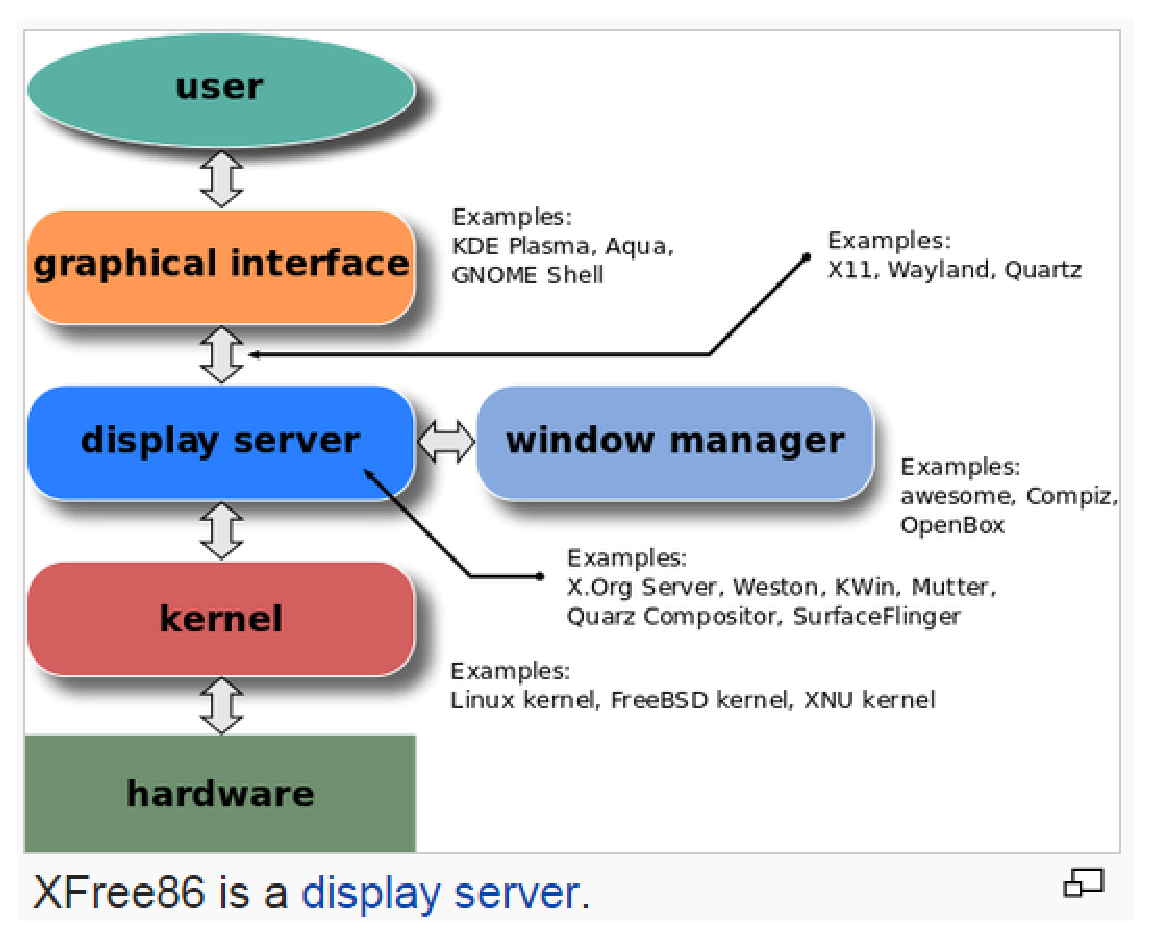
\includegraphics[height=5cm,
    angle=0]{./images/XFree86.eps}}
\caption{XFree86 is a display server}
\label{fig:XFree86}
\end{figure}

\begin{framed}
  XFree86 is the open-source implementation of X11-based desktop
  infrastructure in the form of client-server that provide a
  connection between the window manager (KDE, GNOME...) with the
  hardware (mouse, keyboard, video
  display...)\footnote{\url{http://www.xfree86.org/}}. 
\end{framed}

An early project to integrate accelerated 3D into XFree86 3.3 was called Utah
GLX. Another effort to develop hardware driver for the XFree86 was carried out
by Precision Insight, Inc. (PI) through contracts with various IHVs and ISVs. PI
began the development of the OpenGL DRI ({\bf Direct Rendering Infrastructure})
- the foundation for 3D graphics support on Linux.
The primitive architecture of Utah GLX makes it slower than the DRI but it is
much simpler to implement and is also easier to write drivers for.
\url{http://dri.freedesktop.org/wiki/UtahGLX/} 

The DRI was designed to be flexible in order to accomodate a variety of hardware
architectures. Since the hardware designs are changing and growing more
sophisticated the DRI will also evolve to accomodate these changes.

As of mid-2000 the DRI has been incorporated into XFree86 4.0 and at least five
distinct hardware device drivers have been developed. XFree86 4.0 introduced a
new device driver interface called XAA which should allow XFree86 drivers to be
backward compatible with future versions of the Xserver,
Fig.\ref{fig:XServer_rendering}(1).


The 3D DRI driver essentially converts OpenGL command sequences
into hardware commands. It then uses the kernel module to transmit the commands
to the hardware. It implements the entire OpenGL rendering pipeline
(Sect.\ref{sec:OpenGL}), as much of it as possible in the user space
while the kernel module does whatever is needed in kernel space.
3D DRI drivers usually reside in the 
\begin{verbatim}
/usr/X11R6/lib/modules/dri/
\end{verbatim} 
directory (or specified via \verb!LIBGL_DRIVERS_PATH! environment variable) with
names of the form \verb!device_dri.so.!

In POSIX-based system, the configuration file of XFree86 is in
\begin{verbatim}
/etc/X11/XF86Config
/etc/X11/XF86Config-4
\end{verbatim}
that includes variables about the screen (monitor), keyboard and graphics card.
 
% X.org is the dominant project now with X.org Server is the implementation of 
% X11.

\subsection{DirectFB}
\label{sec:DirectFB}

DirectFB ({\bf Direct FrameBuffer}) functions like X Window System
(Sect.\ref{sec:X11}). However, DirectFB was designed for embedded systems, which
have smaller memory footprint, Fig.\ref{fig:DirectFB}.

\begin{figure}[hbt]
  \centerline{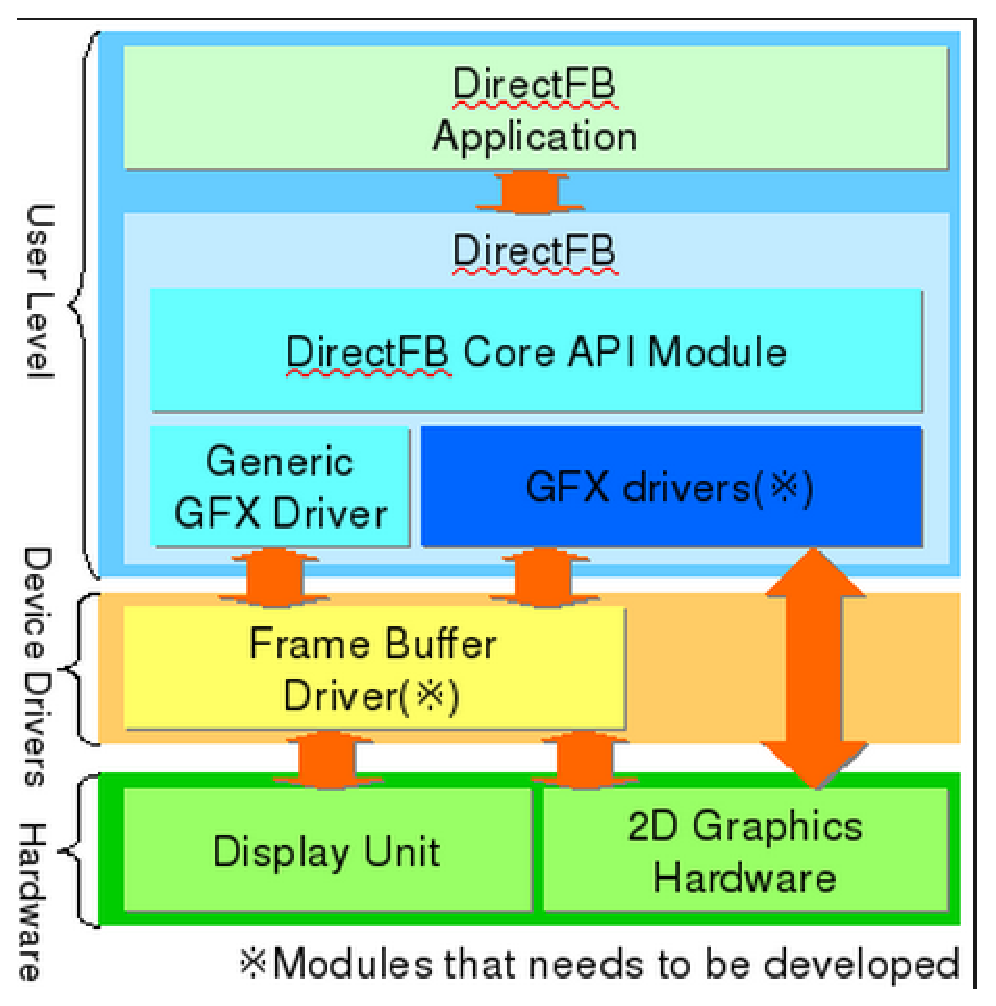
\includegraphics[height=5cm,
    angle=0]{./images/DirectFB.eps}}
\caption{DirectFB}
\label{fig:DirectFB}
\end{figure}


\url{http://stackoverflow.com/questions/3327767/why-is-directfb-not-more-widely-used-in-gnu-linux-are-there-crippling-limitatio}

\subsection{Emulate tools: Xnest, Xephyr}

An X client may emulate an X server by providing a display service
to other X clients. This technique is called {\bf X nesting}. Open-source tools
are \verb!Xnest! and \verb!Xephyr!.

\subsection{Xgl X server}
\label{sec:Xgl}

Xgl is the new XServer architecture layered on top of OpenGL.
It uses two variants of backend implementation, Fig.\ref{fig:Xglx_Xegl} 
to takes advantage of the modern GPUs using OpenGL (Sect.\ref{sec:OpenGL}).
\begin{itemize}
  \item {\bf Xglx}: requires an existing X server and uses GLX
  (Sect.\ref{sec:GLX}) to create an OpenGL window.
  
Xgl must be used in combination with a compositor/window manager to expose all
of its capabilities. Compiz is the compositor utility that was developed in
conjunction with Xgl. Glitz is the key component of the Xgl X server, as it
supports Compiz.

  \item {\bf Xegl}
\end{itemize}
\url{https://tr.opensuse.org/Xgl}

\begin{figure}[hbt]
  \centerline{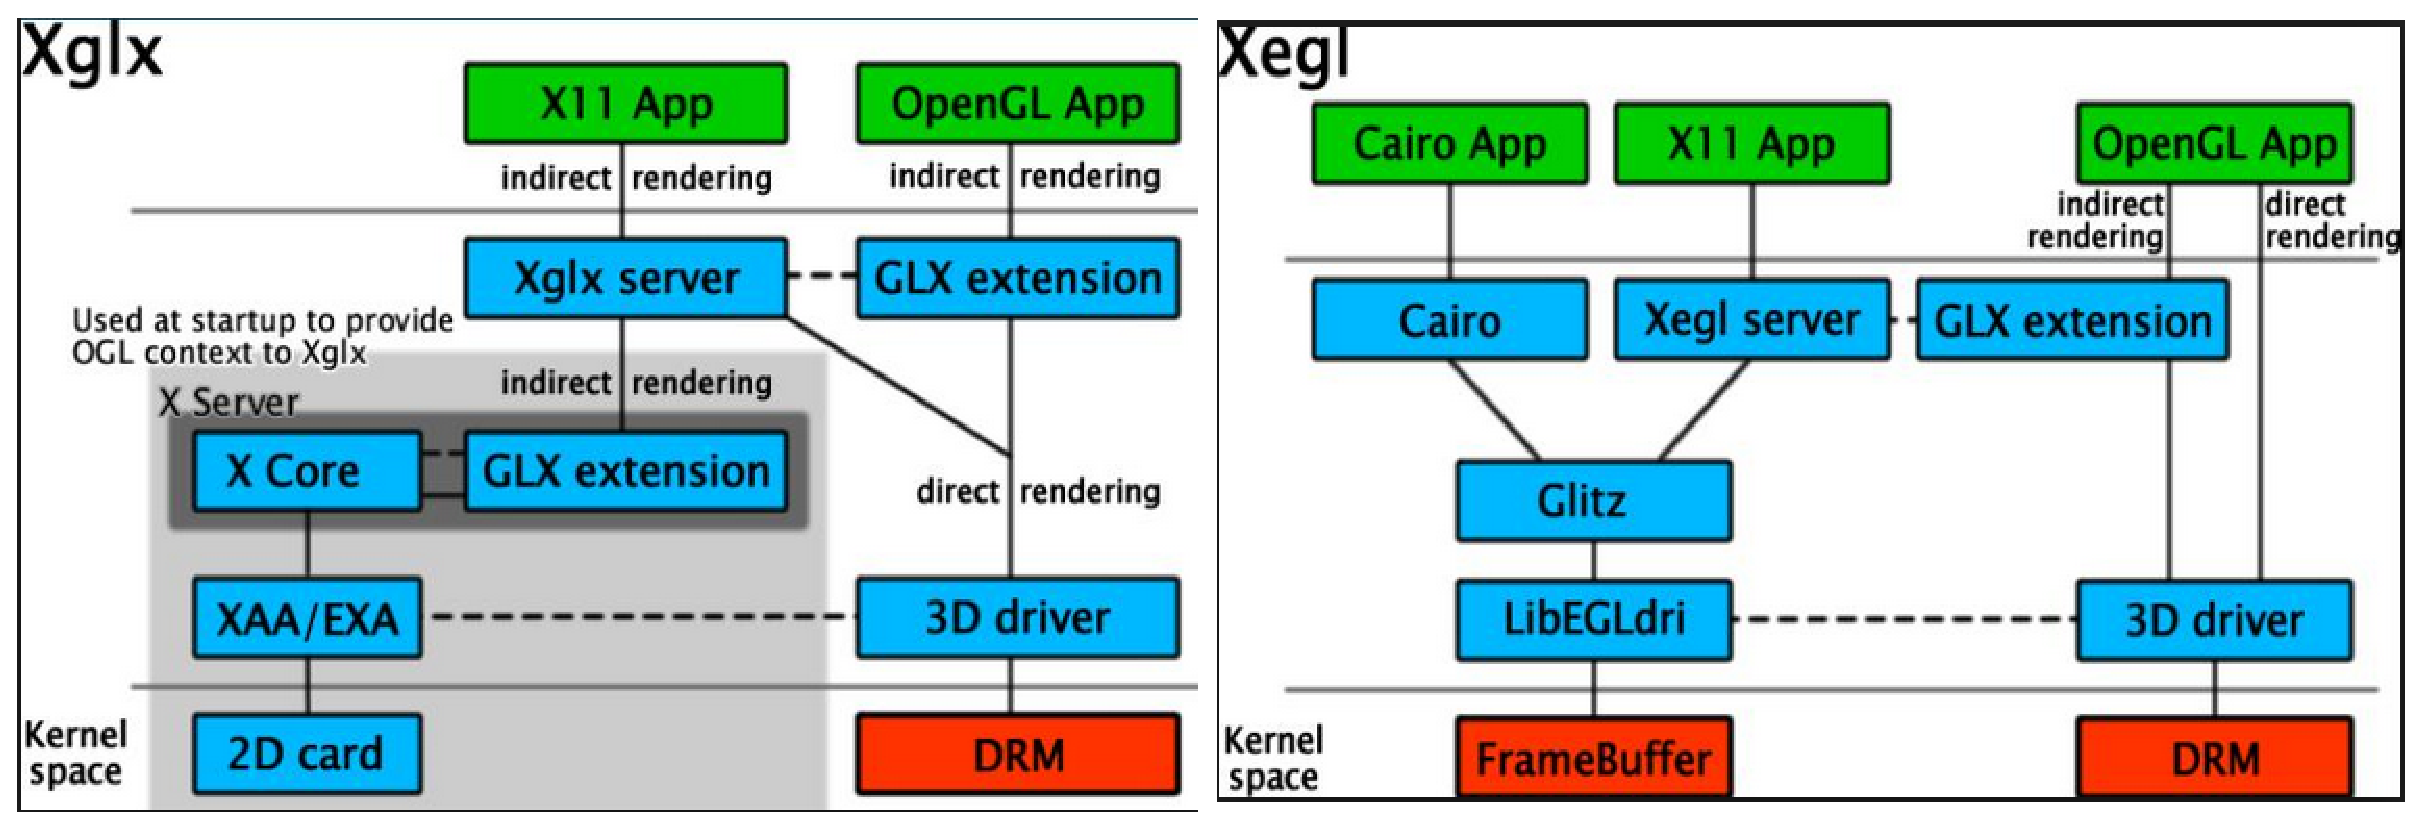
\includegraphics[height=5cm,
    angle=0]{./images/Xglx_Xegl.eps}}
\caption{(A) Xglx server was implemented on top of X Server to provide direct
rendering. (B) Xegl}
\label{fig:Xglx_Xegl}
%http://blog.csdn.net/shallon_luo/article/details/4904769
\end{figure}

%Xgl was first released in 2006, but then was removed in favour of AIGLX.



\section{-- X11's display to Windows}

Suppose you have a headless Linux machine, and you want to display the GUI from
that Linux machine (running X11 server -
Sect.\ref{sec:X-server-implementation}) on a Windows machine. There are several
options:

\begin{enumerate}
  \item VcXsrv - Sect.\ref{sec:VcXsrv} - work best on Windows 64-bit O/S.
  
  
  \item Cygwin/X - Sect.\ref{sec:Cygwin/X}
  \item Xming - Sect.\ref{sec:Xming}
  \item WeirdX - Sect.\ref{sec:WeirdX}
\end{enumerate}

\subsection{VcXsrv}
\label{sec:VcXsrv}

To run Remote X Linux Apps from Windows, for 64-bit Windows 7 and above, you
should consider using VcXsrv Windows X Server.
\begin{itemize}
  \item  MS Windows X11 server based on the Xorg git sources (like xming or
  cygwin's xwin)
  \item actively updated
  \item compiled with VC++ 2012 Express Edition, not 'mingw' making it very MS
  Windows stable.
  
\end{itemize}

\url{https://bbs.nextthing.co/t/need-an-x11-server-for-win7-or-above-vcxsrv-is-based-on-xorg/2882}

\url{https://sourceforge.net/projects/vcxsrv/files/latest/download}


\subsection{MobaXTerm}
\label{sec:MobaxTerm}

MobaXTerm is "sort of" free... it carries its own SSH client and X Display
Server (i.e. client). MobaXTerm is based on Cygwin.

Run MobaxTerm, open Settings/Configuratin, select X11 tab
\begin{verbatim}
Xorg version:
   MobaX
   Cygwin_1.14.5
   Cygwin_1.16.3
   
OpenGL acceleration: Software / Hardware
  --> select Hardware
  
Clipboard: 
  --> select enabled
  
\end{verbatim}


\subsection{Cygwin/X}
\label{sec:Cygwin/X}

Cygwin/X is an implementation of X server on Windows platform. It enables
running a remote/local X11 applications in Windows.

\subsection{Xming}
\label{sec:Xming}

Like Cygwin/X (Sect.\ref{sec:Cygwin/X}), Xming is another implementation of X
server on Windows platform. It is simple and easier to install though less
configurable than other popular free choices like Cygwin/X.

\subsection{WeirdX}
\label{sec:WeirdX}

WeirdX is a pure Java implementation of X Window System server that of course
can run on Windows O/S.
\url{http://sourceforge.net/projects/weirdx/}


\section{ * X11's X client library stack}
\label{sec:X-client-implementation}

An X11 client application is a GUI application, that calls to X11-based APIs
for graphics purpose. There are different libraries that implement X11-based
network protocol APIs. NOTE: The client program can run locally or remotely. 
\begin{itemize}
  \item {\bf Xlib} (Sect.\ref{sec:Xlib}) or 
  
  \item {\bf XCB} (Sect.\ref{sec:XCB})
\end{itemize}
At the bottom level of the X client library stack are Xlib and XCB, two helper
libraries (really sets of libraries) that provide API for talking to the X server. 

Xlib and XCB only provides a set of APIs for the client to tell the server-side
how to render the UI. However, looks-and-feel of the UI components are
implemented by many widget toolkits which built on top of Xlib or XCB,
Fig.\ref{fig:widget_library_system}. So, most likely, you don't have to work
directly with Xlib or XCB, just focus on using Widget toolkits
(Sect.\ref{sec:widget-toolkits-list}).

\begin{mdframed}

How the GUI component looks like (i.e. the visual styling) is not determined by X Window
System. Thus, we can develop the user interface to run on the command-line using
X's graphical capabilities. Also, X provides no native support for audio. 
If we need visual styling, please use Widget toolkits which is a higher level
APIs that enclose calls to these X11 client libraries.
Sparingly, a GUI application may find themselves needing to make calls to the
raw underlying X11 libraries for operations not supported by toolkits.

\end{mdframed}

\subsection{XLib (libX11)}
\label{sec:Xlib}
\label{sec:libX11}

In 1985, {\bf Xlib} library is a X client library, i.e. it provides APIs to
allow the client program to interact with X server easier, by hiding the fact
that calls result in protocol requests to a server. 
\begin{itemize}
  
  \item   Calls that don't require a response from the X server are queued in a
  buffer to be sent as a batch of requests to the server.
  
  \item Those that require a response flush all the buffered requests and then
  block until the response is received.
  
\end{itemize}
Using Xlib is not easy, the thus XCB was developed (Sect.\ref{sec:XCB}).

\begin{mdframed}

Xlib's mix of synchronous and asynchronous behaviors causes some problems.
Xlib's behaviour is often confusing to new programmers. Calls appear to work
sometimes and not others, because it is not obvious which calls implicitly flush
the buffer. The asynchronous nature of many calls makes it difficult to debug
problems. When an error is reported, the stack trace shows the call that was
being made when the error was received and processed, often many calls after the
one that caused the error. Finally, Xlib's synchronous calls incur avoidable
round-trip latency. This latency has a notable effect on application
performance; in particular, startup times are often greatly increased.
\url{https://www.x.org/wiki/guide/xlib-and-xcb/}
\end{mdframed}

Each new extension to the X11 protocol (Sect.\ref{sec:X11}) adds requests that
clients can make to the X server.
Thus, Xlib is aka {\it libX11 for X Window System version 11}. Xlib is written
in C, so Xlib is aka {\it C Library X Interface}. To link to this library, we
pass the following option to the compiler
\begin{verbatim}
-lX11
\end{verbatim}

The programmer needs not know details about X Window System protocol when using
Xlib.
\begin{itemize}
  \item Xlib only provides the API to interact with the X11 Server but does not
  provide any API to implement different GUI components, e.g. buttons or menus.

header file:
\begin{verbatim}
#include <stdio.h>
#include <stdlib.h>
#include <X11/Xlib.h>
#include <X11/Xutil.h>
#include <X11/Xos.h>
#include <X11/Xatom.h>
#include <X11/keysym.h>
\end{verbatim}

  \item APIs provided by Xlib can (1) opening a new window, (2) draw a line, (3)
  write text at a given location in a given window.

As the rendering is taken care by the server-side, Xlib library has no need to
know about the look-and-feel of the UI. 

\end{itemize}

Example: the server is a computer with two video cards, each card can connect to
one or more monitor.  a "display" is a collection of "screens" attached to a
single display device (e.g. a graphics card).

There are 4 important elements in Xlib
\begin{verbatim}
	Display *dis;
	int screen;
	Window win;
	GC gc;
\end{verbatim}


Example: Xlib APIs
\begin{itemize}
  \item XOpenDisplay(), XCloseDisplay

\textcolor{red}{First, connect to the screen which requires the information
about server name and display index (e.g. the graphics card)}
\url{http://tronche.com/gui/x/xlib/display/opening.html}
\begin{verbatim}
Display *XOpenDisplay(display_name)
      char *display_name;
\end{verbatim}  
input can be either a string in the format \verb!hostname:number.screen_number!
\begin{verbatim}
hostname = the machine on which the GUI is displayed
number   = the index of graphic card at 'hostname' (i.e. the display 0 or 1 or
            ???)

screen_number = the index of the screen connected to the
               selected graphics card
               on machine 'hostname'
\end{verbatim}
or NULL (use the string information from DISPLAY environment
variable) 
\url{http://www.pyglet.org/doc/programming_guide/displays_screens_configs_and_contexts.html}

  \item XCreateWindow(), XCreateSimpleWindow()
  
\textcolor{red}{Once the screen is connected, we can request to create a
window}, which returns an {\bf identifiers}, i.e. the client communicate with
the server and ask the server to do specific work for the window of the
given identifier.
\url{http://tronche.com/gui/x/xlib/window/XCreateWindow.html}

% NOTE: XCreateSimpleWindow() requires the screen already connected as it is an
% argument to the function.
\begin{verbatim}
dis = XOpenDisplay(NULL);
win = XCreateSimpleWindow(dis, RootWindow(dis, 0), 1, 1, 500, 500, \
0, BlackPixel (dis, 0), BlackPixel(dis, 0));
\end{verbatim}

  \item XCreateGC()

Graphics context (GC) has a lot to do with how things are displayed/drawn in the
window. Different masks can be set, etc. and you can get pretty funky with it.
\begin{verbatim}
/* create the Graphics Context */
gc=XCreateGC(dis, win, 0,0);    

/* here is another routine to set the foreground and background
	   colors _currently_ in use in the window.
	*/
XSetBackground(dis,gc,white);
XSetForeground(dis,gc,black);
\end{verbatim}
\url{http://math.msu.su/~vvb/2course/Borisenko/CppProjects/GWindow/xintro.html}

  \item XMapWindow()
  
\textcolor{red}{map the created window to the screen}

  \item XGetWindowProperty()
  
  \item XSelectInput()
  
Tell the X Server what kind of event that the program want to process
\begin{verbatim}
XSelectInput (dis, win, ExposureMask | KeyPressMask | ButtonPressMask);
\end{verbatim} 
NOTE: In the event-loop, we will check for the occuring of these event using
operation on the event queue

  \item operation on event queue: XNextEvent(), XPeekEvent(), 
  
XPeekEvent() function returns the first event from the event queue, but
it does not remove the event from the queue
  
Events in X are things like the mouse buttons being clicked, or the keys on the
keyboard being pressed. The events can either be KeyPress or KeyRelease for
keyboard control devices.
 When the window is resized the application is sent a ConfigureNotify event.
When the window is below another window and is raised it is sent an Expose
event, which would usually redraw the application. When the window is initially
created an Expose event is sent.


  \item operations on local dataa: XCreateImage(), XSaveContext(),
  XParseGeometry()
\end{itemize}
  
The main type of data in Xlib are \verb!Display! structure and types of
{\it identifiers} (e.g. \verb!Windows!, \verb!Pixmap!, \verb!Font!,
\verb!Colormap!). Identifiers are 32-bit integers.
\begin{itemize}
  \item Windows, colormaps, etc. are managed by the server, which means that the
  data about their actual implementation is all stored in the server. 
  
  \item The client operates on these objects by using their identifiers. The
  client cannot directly operate on an object, but can only request the server
  to perform the operation specifying the identifier of the object.
\end{itemize}
Most Xlib functions have a Display structure as an argument because they either
operate on the channel or are relative to a specific channel. 

\textcolor{red}{To be able to catch different events, an infinite loop (event
loop) is the common approach in GUI program}. This is called event-driven
application (Sect.\ref{sec:event_driven_app})
\begin{verbatim}

while (1)  {
  XNextEvent(dis, &report);
  switch  (report.type) {
    case Expose:   
      fprintf(stdout, "I have been exposed.\n");
/*A local program function to redraw the window should be called.*/
    break;
    }
  
  
    if (event.type==KeyPress&&
		    XLookupString(&event.xkey,text,255,&key,0)==1) {
		/* use the XLookupString routine to convert the invent
		   KeyPress data into regular text.  Weird but necessary...
		*/
			if (text[0]=='q') {
				close_x();
			}
			printf("You pressed the %c key!\n",text[0]);
		}  
}

\end{verbatim}

\textcolor{red}{Finally, implement the function to free memory once the program
exit}
\begin{verbatim}
void close_x() {
/* it is good programming practice to return system resources to the 
   system...
*/
	XFreeGC(dis, gc);
	XDestroyWindow(dis,win);
	XCloseDisplay(dis);	
	exit(1);				
}
\end{verbatim}


Example: A client 'creates' a window by requesting that the server create
a window. This is done via a call to an Xlib function that returns an identifier for the
window, that is, a number. The client then use this identifier for requesting
other operations on the same window to the server.

The Xlib functions that send requests to the server usually do not send these
requests immediately but store them in a buffer, called the
\textcolor{red}{\bf request buffer}. 
The request buffer can contain all kinds of requests to the server, not only
those having a visible effect on the screen. 
The request buffer is guaranteed to be flushed (i.e., all requests done so far
are sent to the server) after a call to the functions \verb!XSync! or
\verb!XFlush!.

NOTE: The X Server returns \verb!events! to the Xlib which stores them in a
queue. While the X server sends events asynchronously, applications using the
Xlib library are required to explicitly call Xlib functions for accessing the
events in the queue.
\url{http://en.wikipedia.org/wiki/Xlib}

Example:
\begin{verbatim}
#include <X11/Xlib.h>

int main(void)
{
    Display *display;
    Window window;
    XEvent event;
    int s; // identifier
    
     /* open connection with the server */
    display = XOpenDisplay(NULL);
    
    s = DefaultScreen(display);
    
    /* create window */
    window = XCreateSimpleWindow(display, RootWindow(display, s), 10, 10, 200, 200, 1,
                           BlackPixel(display, s), WhitePixel(display, s));
 
    /* select kind of events we are interested in */
    XSelectInput(display, window, ExposureMask | KeyPressMask);
 
    /* map (show) the window */
    XMapWindow(display, window);
    
    
    /* event loop */
    for (;;)
    {
        XNextEvent(display, &event);
 
        /* draw or redraw the window */
        if (event.type == Expose)
        {
            XFillRectangle(display, window, DefaultGC(display, s), 20, 20, 10, 10);
            XDrawString(display, window, DefaultGC(display, s), 50, 50, msg, strlen(msg));
        }
        /* exit on key press */
        if (event.type == KeyPress)
            break;
    }
 
    /* close connection to server */
    XCloseDisplay(display);

   return 0;
}
\end{verbatim}

\subsection{XCB (libxcb)}
\label{sec:XCB}
\label{sec:libxcb}

XCB (X protocol C-language Binding) - aims to replace Xlib (libX11).

XCB makes the client-server nature of the protocol explicit in its design. The
client is in charge of deciding when to flush the request buffer, when to read
results and when to wait for the server to respond.



\subsection{Xlib/XCB}

Xlib/XCB is the modern choice which implement Xlib on top of XCB library, i.e.
rebuild libX11 as a layer on top of libxcb. 

One can use Xlib to open the display and pass the Display pointer it returns to
existing code, toolkits, and libraries. To call an XCB function, one can convert
the Display pointer to an \verb!xcb_connection_t! pointer for the same
connection.
This enables calling into Xlib and XCB from the same application.
Xlib and XCB share the same X server connection and pass control of it back and
forth. That option was introduced in libX11 1.2, and is now always present (no
longer optional) since the 2010 release of libX11 1.4.




\section{Mir}
\label{sec:Mir}

{\bf Mir} is a  display server (Sect.\ref{sec:display-server}) for the Linux
operating system that is under development by Canonical Ltd since 2013.

The goal to have Mir is to have lower overhead in the display pipeline, more
seamless transitions between display modes during the boot process, richer input
handling that will make it easier to support things like touchscreen gestures,
more seamless support for systems with switchable graphics hardware (like
laptops that can dynamically shift between using embedded and discrete
graphics), and better application interchange (which will help improve things
like the clipboard and drag-and-drop).

\begin{enumerate}
  \item Unity 8 has native support for Mir
  
  \item 
\end{enumerate}
The compatibility layer for X, XMir, is based on XWayland.



\section{History of 2D graphics library in Windows}
\label{sec:2D-graphics-Windows}

\subsection{Port X-Windows System to Windows}

There are different implementation that allows displaying the UI of a
programming running on a 'remote' X-Windows system on Windows.

{\bf X-Win32} a proprietary implementation of the X Window System for Microsoft
Windows, based on X11R7.4. It allows a remote Unix program to display on Windows
local machine. \url{http://en.wikipedia.org/wiki/X-Win32}

{\bf Cygwin/X} is a free alternative to provide a similar featuer as X-Win32,
and is part of the Cygwin project (Sect.\ref{sec:Cygwin/X}).
Cygwin/X was originally based on XFree86 (Sect.\ref{sec:XFree86}), but
has been switched to the X.Org Server since the discontinuing of XFree86
project.
\begin{itemize}
  \item provide an X Server environment to run GUI application from Cygwin
  \item provide an X Server environment to run GUI application from a remote
  Linux machine. Protocols it supports: XDM, SSH tunneling.
\end{itemize}

{\bf Xming Server} a proprietary implementation based on Cygwin/X and X.Org
Server. Protocols for remote connection: SSH X11 forwarding, PuTTYs

{\bf Xwin} - a strip-down version of Cygwin/X, just for running X Server in
Windows. \url{http://wiki.dennyhalim.com/xwin}

\subsection{GDI (16-bit): use DC (device context) objects}
\label{sec:GDI}
\label{sec:DC-device-context}

To provide the UI to a program running on Windows, GDI was introduced since the
first version of Windows. GDI is a C library and is 16-bit library. On 32-bit
platform, it is replaced by Win3 GDI (Sect.\ref{sec:Win32GDI}).

The goal of developing GDI is to provide a device-independent API, i.e.
a program written using the GDI will work on all graphics and printer hardware,
provided suitable Windows GDI drivers for the hardware are installed on the
system. 

A common device-independent approach is to write data (graphics (bitmaps)) to a
logical graphics {\bf device context} (DC), but not to the physical framebuffer
on the hardware directly.
\textcolor{red}{The major limitation of the GDI DCs was that they were {\bf
write-only}}. Data, once written, could not be retrieved.
This was because the contents of the DC was device dependent, and data read from
it would make no sense to the programmer.

A {\bf bitmap} is the in-memory representation of the picture to be drawn on the
drawing surface of the DC. GDI also has a number of functions that can copy
areas from the drawing surface of one DC to another, so bitmaps then are a
useful way to store images in memory that will later be copied to the display
(or other devices).

The DC is then translated by the GDI and the device drivers to suit the target
hardware device and is written to its physical frame buffer in an appropriate
manner
\begin{itemize}
  
  \item A {\bf Device Context} (DC) is a handle to a drawing surface on some
  device - Device Contexts can typically be obtained for the display device (the
  entire screen), printers and plotters.
  
Most commonly worked with are {\bf window DC} (a display DC that merely
represents the area of a single window) and a {\bf memory DC} that represents a
bitmap as a device.

  \item For a given DC, a number of tools that can be used to act on the
  associated drawing surface: Pens, brushes, fonts, etc.
  
In the case of memory DC, a number of preset pens are provided, and more can be
created on the fly as needed.
\end{itemize}

%GDI is too slow for animation, as it cannot access hardware directly.
In order to do animation using the GDI DC, all of the animation frames needed to
be manipulated in system memory and then each frame needed to be copied into a
GDI DC for display on the graphics device. This was a very slow process.

\url{http://www.codeproject.com/Articles/356/Bitmap-Basics-A-GDI-tutorial}

\subsection{DCI (Device Control Interface)}
\label{sec:DCI}

\url{http://stason.org/TULARC/pc/video-faq/54-What-is-DCI.html#.VOWN_fnF_Xo}

Unlike GDI, which doesn't write data directly to hardware graphics bufer, DCI
was developed to enable that feature, i.e. faster. The goal was to support
video games that require fast rendering.
DCI is replaced by DirectDraw (Sect.\ref{sec:DirectDraw}).

DCI stands for "Device Control Interface." It's an Intel/Microsoft standard, and
exists primarily as a way for Windows 3.1 to exploit the video acceleration
features of a graphics card, and/or to provide fast video when needed. 

A DCI driver exists at the same software layer as the GDI.
Thus, support for DCI features doesn't need to be in hardware -- a graphics card
vendor could provide a DCI driver that allowed Windows 3.1 apps to speak DCI,
but the graphics card could be performing the DCI functions with a software
driver.

Among DCI's capabilities are the ability to {\it write directly to the frame
buffer} (helpful for high-speed games) and the ability to provide for on-board
hardware acceleration of video scaling (i.e. stretching a video window to a
larger size) and color space conversion (converting the YUV format color
information in a video file to the RGB format that a typical graphics card
RAMDAC expects).


\subsection{WinG (Win 3.x): WinGDC}
\label{sec:WinG}

As the original GDI was designed with static image in mind, it is not suited for
video (games). WinG APIs was developed as a quick-fix to GDI API.
WinG APIs was used in Windows 3.x, and until Windows 95, Windows 98 and Windows
NT 4.0; and stopped since Windows 98 Second Edition, Windows 2000, due to the 
inception of DirectX (Sect.\ref{sec:DirectX}).

% NOTE: DC in GDI is write-only. 
% 
Using the DC concept similar to GDI (Sect.\ref{sec:GDI}), WinG introduced a new
type of device context called {\bf WinGDC} that uses DCI (Sect.\ref{sec:DCI})
and thus allowed programmers to both read and write to it directly using DIB
(device-independent bitmap) with \verb!wingdib.drv! driver.

This meant that fast graphics algorithms could be written to allow fast
scrolling, overdraw, dirty rectangles, double buffering, and other animation
techniques.
WinG also provided much better performance when blitting graphics data to
physical graphics device memory.

WinG would also perform a graphics hardware/driver profiling test on the first
execution of the program in order to determine the best way to manipulate the
graphics hardware.
Once WinG had determined the fastest calls that did not cause graphics
corruption, a profile would be saved so that the test would not need to be
performed again.


\subsection{Win32 GDI (32-bit)}
\label{sec:Win32GDI}

In Windows, Win32 GDI (Graphics Device Interface) is the GDI library for graphics
model from Windows 95 and is supported on all 32-bit Windows (Win32) platforms.
When we say Win32, it means Win32 GDI. Win32 GDI is still a C library. 
A better replacement is DirectWrite (Sect.\ref{sec:DirectWrite}). 

\begin{mdframed}

GDI a low-level library and is responsible for tasks such as drawing lines and
curves, rendering fonts and handling palettes.
GDI is NOT responsible for drawing windows, menus, etc. These tasks are served
for APIs in \verb!user32.dll! libraries.

Thus, GDI is relatively hard to use for advanced animation, and lacks a notion
for synchronizing with individual video frames in the video card, lacks hardware
rasterization for 3D, etc.
\end{mdframed}

%A better replacement is OpenGL and DirectX.


\subsection{GDI+ (32-bit, C++): Windows XP}
\label{sec:GDI+}

GDI+ is C++ library to complement GDI C-based library since Windows XP.
GDI/GDI+ is replaced by Direct2D (Sect.\ref{sec:Direct2D})

GDI+ is an improvement on GDI with features not readily available
in GDI such as 
\begin{enumerate}
  \item gradient brushes, 
  
  \item alpha blending, and 

  \item GDI+ uses  ARGB values to represent color.

 \item anti-aliased 2D graphics, 
 
 \item floating point coordinates,

  \item gradient shading, 
  
  \item more complex path management, 
  
  \item more image format support: intrinsic support for modern graphics-file
  formats like JPEG and PNG, and support for composition of affine
  transformations in the 2D view pipeline.
 
\end{enumerate}
\url{http://stackoverflow.com/questions/4551224/what-is-the-difference-between-gdi-and-gdi}

NOTE: GDI+ is nearly an order of magnitude slower than GDI, but that's not too
big of an issue on modern machines with more power than you could ever want. 
%This, too, is going to be supported for a very long time to come.

The Microsoft .NET class library provides a managed interface for GDI+ via the
\verb!System.Drawing! namespace.

GDI+ continues to rely on software rendering in Windows 7.

\subsection{GAPIDraw (Graphics API - Windows Mobile)}
\label{sec:GAPI}

The Graphics API (GAPI) was a technology that allow  creation of
high-performance graphical applications across a variety of handheld hardware
configurations, including Palm, Symbian and Windows Mobile devices.
GAPI means Game    Application    Programming    Interface    for    
Drawing, and was originally designed for game development.
\url{http://dl.acm.org/citation.cfm?id=1052388}

It borrows many features from DirectX.
GapiDraw API is a mix between a Frame-Buffer API (i.e. draw using CPU) and a 
Graphic  Hardware  API (i.e. draw using GPU). GAPI was replaced by DirectDraw
(Sect.\ref{sec:DirectDraw}) since Windows Mobile 5.0. No maintainance for
backward compatibility since Windows Mobile 6.5.

GABI contained functions that allowed an application to request all button press
messages, even the ones that were normally intercepted by the Windows Mobile
operating system. This function is
\begin{verbatim}
 GXOpenInput()
\end{verbatim}
 
GAPI is using a DRAM buffer, i.e. you cannot write directly in the raw frame
buffer with GAPI, rather GAPI GXBeginDraw will return you the address of a
176x220 memory buffer, which will be copied in the real display frame buffer
when you call GXEndDraw.
\url{http://www.modaco.com/topic/241988-gapi-on-the-motorola-q-what-developers-need-to-know/}

 
\subsection{DirectDraw (part of DirectX on Windows Mobile)}
\label{sec:DirectDraw}

DirectDraw is 2D API, supports hardware acceleration and was used since
Windows Mobile 5.0. NOTE: For 3D rendering, read Sect.\ref{sec:Direct3D}

DirectDraw was then merged into a new package of {\bf DirectX 8.0} called
{\bf DirectX graphics} to extend Direct3D with DirectDraw APIs.

The header files and DirectDraw library is no longer included in DirectX SDK
since June-2010. Since DirectX 9.0, it is recommended to use Direct3D
(Sect.\ref{sec:Direct3D}) as you can do everything you want from DirectDraw, as
well as get better hardware acceleration and be able to add traditional 3D
related features (texture mapping, etc).

\verb!AllKeys()! is the keyboard API function to use in place of GAPI keyboard
function. 

IMPORTANT: \verb!AllKeys! exists as long as GAPI and GAPI
\verb!Gx(Open/Close)Input()! keyboard function is just a wrapper to this
function.

\begin{verbatim}
 GXOpenInput() with AllKeys(TRUE).
 
 GXCloseInput() with AllKeys(FALSE).
\end{verbatim}

Syntax:
\begin{verbatim}
BOOL AllKeys(

     BOOL bAllKeys

);

Nonzero indicates success. Zero indicates failure. To get extended error
information, call GetLastError.
\end{verbatim}
If bAllKeys is set to TRUE, this function allows all keyboard events to be sent
to the application. (This includes the soft-key buttons and back button).

If it is set to FALSE, this function specifies standard keyboard event behavior.
Some events including soft-key buttons and the back button are not sent to the application.

Example:
\begin{verbatim}
// process checkbox

case IDC_ALL_KEYS_CHECK_BOX:

if (g_AllKeys == true)

    {

    // Allow the OS to intercept some button presses

     AllKeys(FALSE);

    g_AllKeys = false;

    // set button state

    SendMessage(hwndCtl,BM_SETCHECK, BST_UNCHECKED,0);

    }

else

    {

    // Do not allow os to intercept button presses

    AllKeys(TRUE);

    g_AllKeys = true;

    //set button state

    SendMessage(hwndCtl,BM_SETCHECK, BST_CHECKED,0);

    }
\end{verbatim}

\subsection{Direct2D}
\label{sec:Direct2D}


\subsection{Uniscribe (text rendering)}
\label{sec:Uniscribe}

Uniscribe provides services for rendering Unicode-encoded text, especially
complex text layout. The library is \verb!USP10.dll! and is used in Windows
2000, Windows CE 5.0.

Uniscribe is replaced by DirectWrite since Windows 7
(Sect.\ref{sec:DirectWrite}).

\url{http://en.wikipedia.org/wiki/Uniscribe}

\subsection{DirectWrite (text rendering)}
\label{sec:DirectWrite}

DirectWrite is a text layout and glyph rendering API.
DirectWrite is designed to replace Uniscribe (Sect.\ref{sec:Uniscribe}) for
screen-oriented rendering and was shipped with Windows 7, Windows Server 2008 R2, \ldots

DirectWrite is hardware-accelerated when running on top of Direct2D
(Sect.\ref{sec:Direct2D}), but can also use CPU.




\section{History of 2D graphics library in Mac OS/X}

Developers for Mac O/S decided not to use X11; but Quartz
(Sect.\ref{sec:Quartz}). The reason was that so many features they needed was
not available in X11, and they decided to implement a whole new windowing
system. 

Back then, X didn't have any kind of compositing model and Quartz was better.
In terms of current capabilities, Quartz and a recent version of X.org are
similar. The difference is that X.org has a cleaner separation of policy and
mechanism, and maintains backwards compatibility with applications dating back
to the mid 1980s
 

\subsection{QuickDraw: used on MacOS Classic systems}

 QuickDraw, found on the old MacOS Classic systems, was a very simple design.
One process mediated access to the display, allocating regions to other
processes, and the other processes drew into these directly.

The obvious disadvantage to this was that all processes had access to the frame
buffer, so could corrupt the display easily and synchronizing drawing between
applications was very difficult.

\subsection{Display PostScript: NeXT systems}

Processes on old NeXT systems sent PostScript programs to the display server,
which then ran them. This had its own problems, such as the fact that the
display server effectively needed to be a complex multitasking virtual machine
to prevent programs from taking over all of the display's time.



\subsection{Quartz}
\label{sec:Quartz}

The design of Quartz was simple.
Just as a filesystem virtualizes the disk by providing virtual disks (files) to
applications, Quartz virtualizes the screen by providing virtual frame buffers
(windows) to applications. This is the Quartz Compositor or simply the 'Window
Server,'. The window server provides a region of shared memory to clients for
drawing and then composites this into the frame buffer (on the GPU).
It's a little bit more complicated than that, because this buffer is now an
OpenGL texture and can be the result of rendering OpenGL graphics to the texture
or compositing other textures together.


In Mac OS, Quartz is the graphics model.
\begin{itemize}
  \item Quartz 2D: 2D text and graphics rendering library

Since Mac OS X 10.4, Quartz 2D Extreme, which allows Quartz 2D to use supported GPUs for rendering.
As of Mac OS X v10.5 Quartz 2D Extreme has been renamed to QuartzGL.

\url{http://en.wikipedia.org/wiki/Quartz_(graphics_layer)}
  
  \item Quartz compositor: the compositing engine
  (Sect.\ref{sec:compositing_engine}). 
  
  It is used by Quartz 2D, OpenGL, Core Image, QuickTime.
  
  Since Mac OS X 10.2, Quartz Compositor uses GPU directly to improve composition performance.
    
\end{itemize}

% \section{X Window System vs. Quartz vs. Win32 GDI}
% 
% X Window System is the implementation for client-server communication in Linux.




\section{History of 2D/3D graphics library}
\label{sec:3D_graphics-library}

CRT monitors were first used to display ASCII text. Then, they are
used for displaying lines and points which can be combined to form
more complicated geometric shapes. In 1970s and 1980s, there is a
science of creating algorithms for efficiently creating lines and
curves on the display. These first computer graphics are 2D, with libraries
implemented the algorithms that we have introduced in the earlier sections
(Sect.\ref{sec:2D-graphics-Windows}, Sect.\ref{sec:2D-graphics-Linux}).

Then, there is a demands of producing animation or a sequence of
images that they call {\it real-time} in response to some input
(keyboard, mouse, joystick...) which is largely used in computer
games. At it was only 2D graphics, and then 3D graphics was developed to provide a
more visual-realistic perspective to the graphics (image, video).

Since the X11 standard was much earlier, it has no 3D features (until some
efforts - Sect.\ref{sec:X11-3D}), so OpenGL has become the common way of
providing these. The OpenGL standard (Sect.\ref{sec:OpenGL}) is an API defining
an abstract 3D language (the other common API being Microsoft's Direct3D -
Sect.\ref{sec:Direct3D}).

\textcolor{red}{In Linux, the APIs for graphics handling is not part of the O/S
kernel}. Initially, in Linux, X Server directly managed the resources of GPU
(Sect.\ref{sec:XServer}) via the 2D driver inside X Server,
Fig.\ref{fig:XServer_rendering}(1). To enable OpenGL application running on X
Server, Utah GLX was implemented using GLX protocol (Sect.\ref{sec:GLX}),
Fig.\ref{fig:XServer_rendering}(2).

\begin{figure}[hbt]
  \centerline{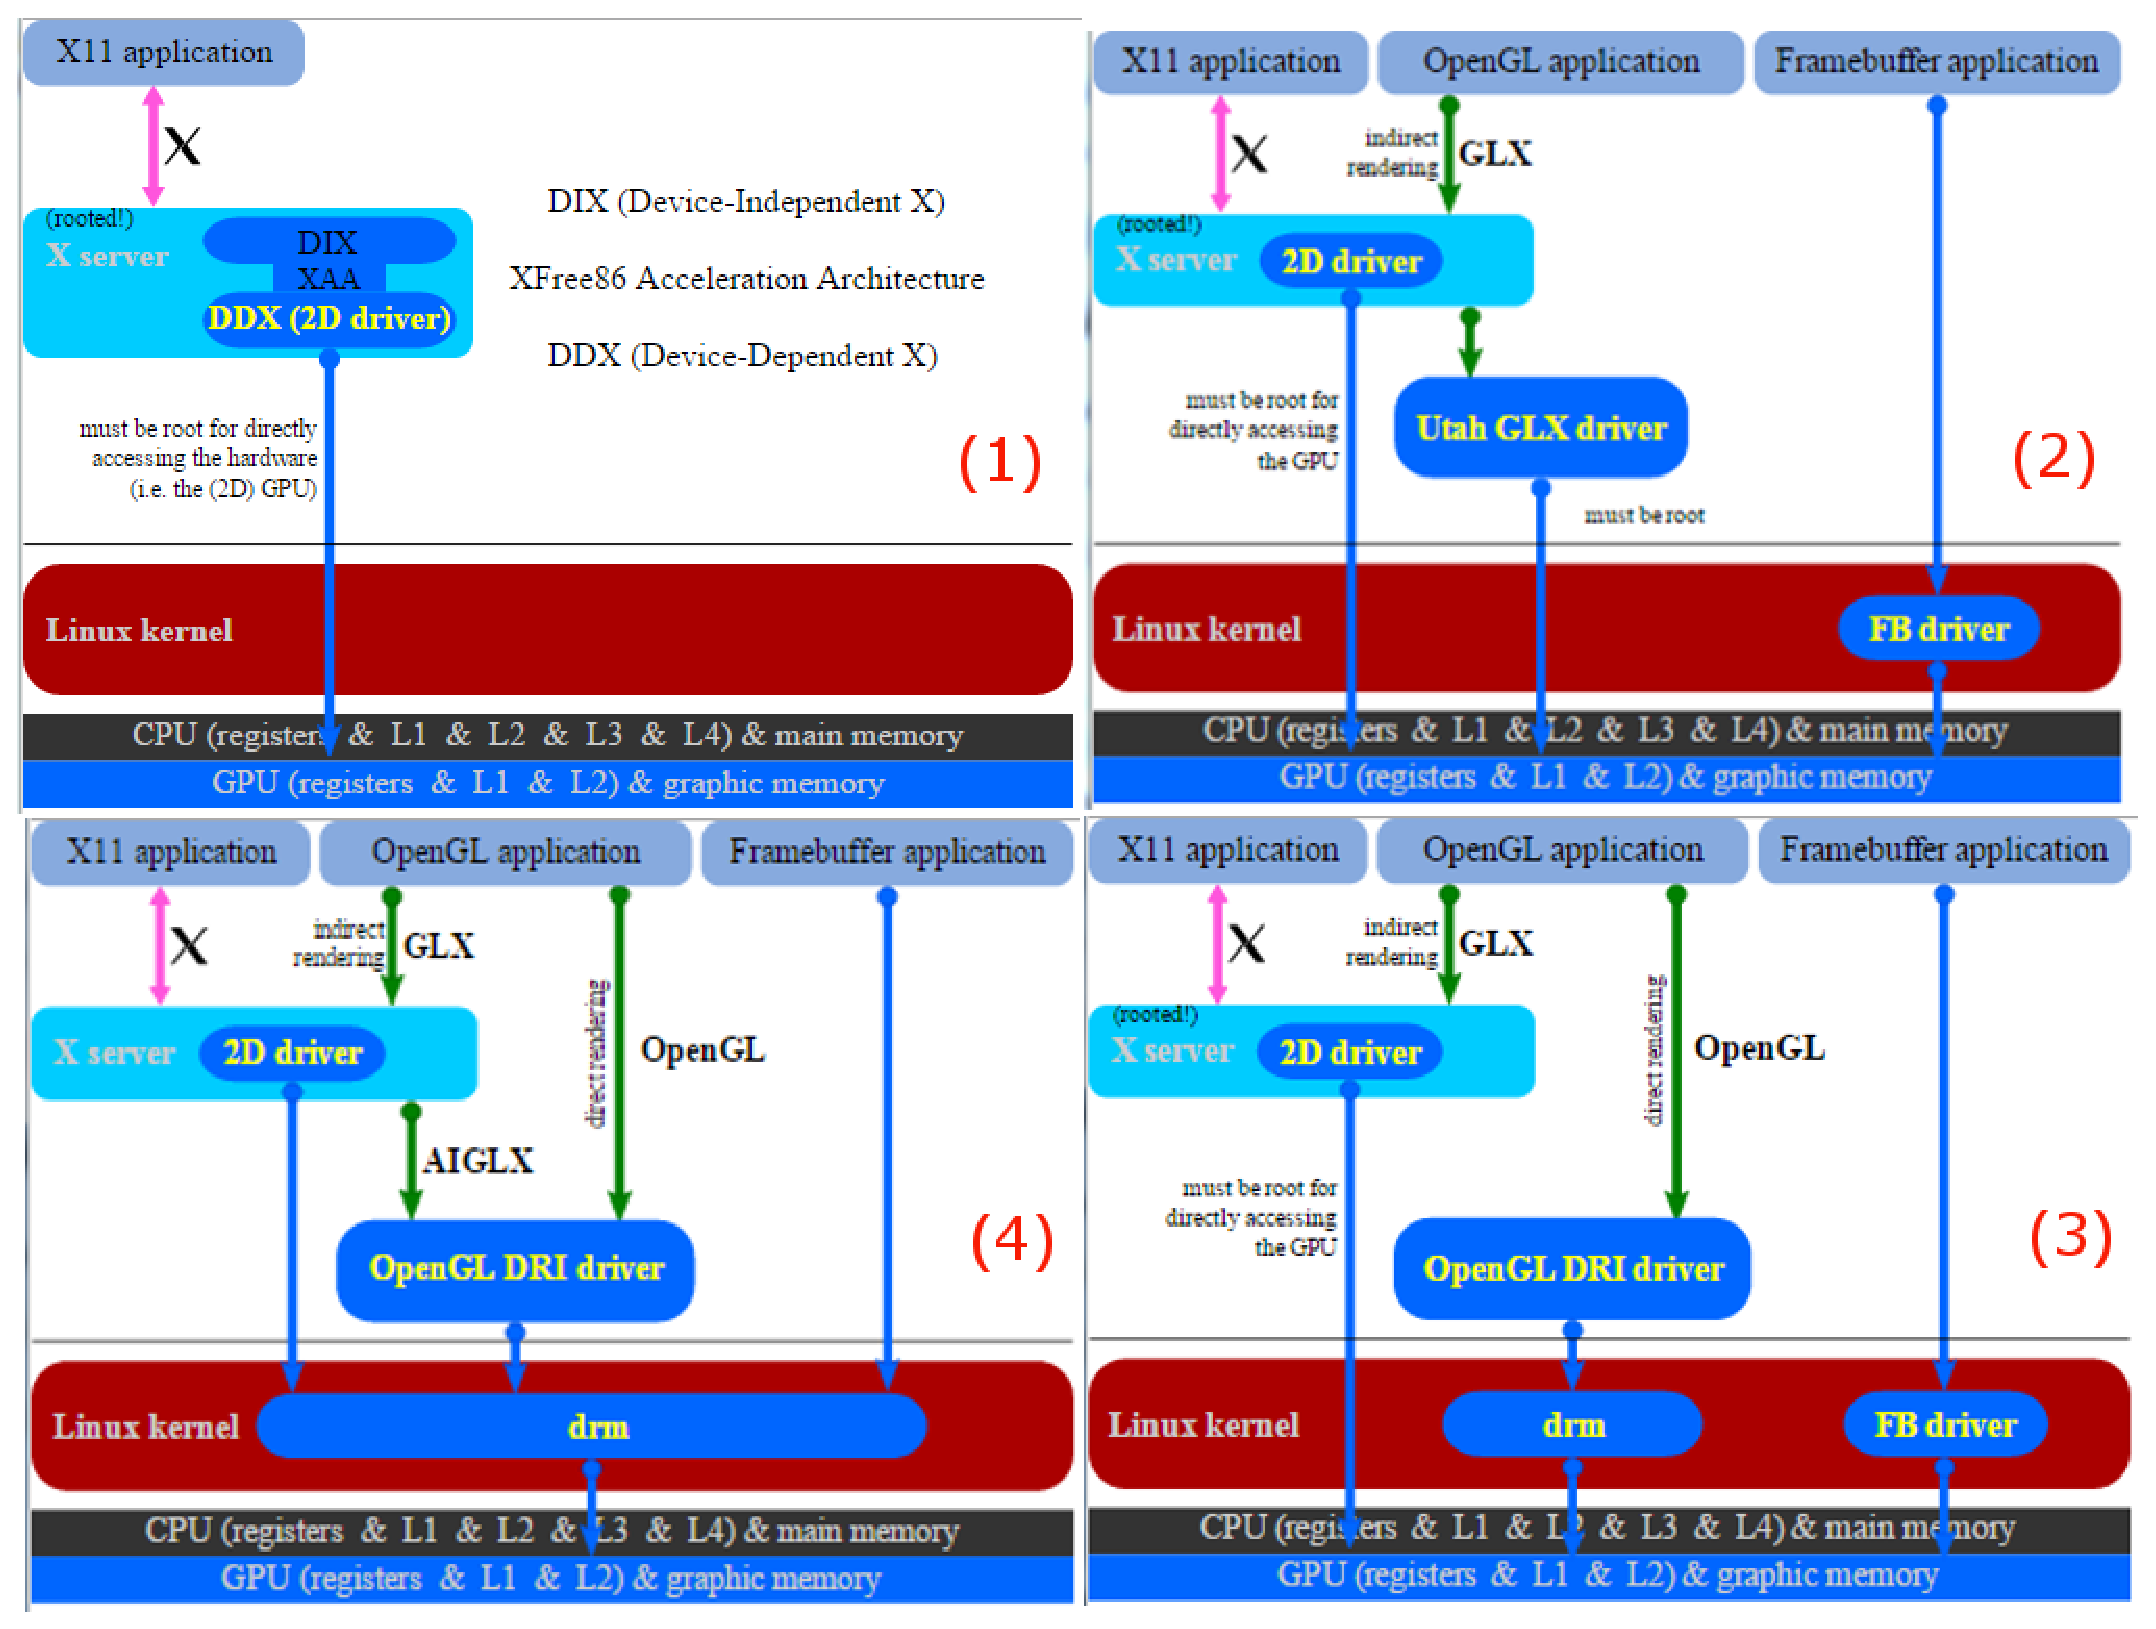
\includegraphics[height=10cm,
    angle=0]{./images/XServer_rendering.eps}}
\caption{Different rendering techniques at different versions of X Server: (1)
2D driver inside X Server (DDX = XFree86 2D), (2) Utah GLX for 3D indirect
direct rendering of OpenGL applications, (3) Early DRI architecture with OpenGL DRI driver, (4) DRM
controls all direct access to graphics hardware}
\label{fig:XServer_rendering}
\end{figure}



\subsection{What is 3D graphics: perspective and surface
lighting/shading, texture mapping, blending}

3D refers to objects that have width, height and depth. However, in
computer graphics, they are displayed on 2D monitor. So, it requires
algorithms for projecting ... in such a way that provide an illusion of
depth. This is known as {\bf perspective} (\verb!glPerspective()!
which tells the angle between the lines that tells the illusion of
depth).

However, perspective is not enough to provide you a true 3D
feeling. Another information that you need is {\it surface shading}
due to lighting, and the relative size of different objects.
This is known as {\bf foreshortening}. 

\begin{framed}
  In summary, all that we need to create 3D feeling are perspective,
  foreshortening, color change, texture, shading and variation of
  color intensities. 
\end{framed}

The process of transforming a mathematical and image data into 3D
image on the display is called {\bf rendering}. One of the process in
rendering is {\bf transformation and projection}. 
\begin{itemize}
\item transforming = moving the points (i.e. {\bf vertices}) around so
  that the line connecting them produce the illusion of a 3D world on
  a 2D display. To move the points, we need a {\bf transformation
    matrix}, and to convert the 3D coordinates onto a 2D display, we
  need another matrix - called {\bf projection matrix}. 
\end{itemize}

2D display is indeed a matrix of pixels. So, to make a line, we need
to fill the pixels with appropriate colors. This process is known as
{\bf rasterization}. One technique often used during this process is
{\it hidden surface removal}. Not only lines (i.e. wireframe
rendering), but also solid geometric primitives (triangles, polygons)
are also rasterized, i.e. we need to fill color on a surface, not only
a single line. OpenGL provides APIs for filling colors into geometric
primitives.

\begin{framed}
  Primitives are one- or two-dimensional entities or surfaces like
  points, lines, triangles, polygons that are assembled into a 3D
  space to form 3D objects.

  A vertex is nothing more than a coordinate in 3D, with
  color/normal/... information. Creating a solid 3D geometry is little
  more than a game of ``connect-the-dots''. 
\end{framed}

In addition to filling a solid color, there is a need of {\bf
  shading}, i.e. varying the color across the surface. This will
create the effect of light shining on a red cube. 
\textcolor{red}{Lighting and shading is a major part in 3D computer
  graphics}. 


Not only filling the color on a surface, you may want to fill it using
a given picture. This is known as {\bf texture mapping}. This adds a
whole new level of realism to our rendering. 

Another level of realism is {\bf blending}, which allows you to add
``mirroring'' effect, i.e. transparency. 


\subsection{Real-time vs. Non-real-time 3D}
\label{sec:real-time-vs}

In real-time, your input cause a change in the 3D visualization within
an unnoticeable time. 

In non-real-time 3D, normally the result is very high quality
image. So, rendering a single frame may need lots of computational
processing, and thus time. In 3D movies, ones design the models and
scenes or ones can use a program (Maya, ...) to create the content,
then the results is sent to a ray tracer (scan-line renderer) to
generate the 3D images.  Thousands of frames are generated and then
combined to form a 3D movies, though the content is not interactive.
\subsection{X11 - 3D: GLX, DRI}
\label{sec:X11-3D}

Direct graphics hardware access support for X Server started with 3dfx GlideAPI
in the Mesa implementation for Voodoo GPU (Sect.\ref{sec:mesa-3d}).

There was another effort to develop hardware driver for the alternative X Server
implementation, XFree86 (Sect.\ref{sec:XFree86}), that lead to
the {\bf Direct Rendering Infrastructure} (DRI) - the foundation for 3D graphics
support on Linux. 

To help resolve the problem with two programs trying to control the same video
card at the same time, the {\bf drm} component (Direct Rendering Manager) was
added to the Linux kernel, Fig.\ref{fig:XServer_rendering}(3)(4).

The DRM gets an exclusive access to the video card, and it's responsible for
initializing and maintaining the command queue, the VRAM and any other hardware
resource. The programs that want to use the GPU send their requests to DRM,
which acts as an arbitrator and takes care to avoid possible conflicts.
\url{http://en.wikipedia.org/wiki/Direct_Rendering_Manager}

\subsection{ -- GLX}

GLX provides extensions to X11 to provide this functionality, ie taking client
OpenGL calls and passing them on to the OpenGL libraries, which can also involve
encapsulating these commands to be passed across a network connection.


\subsection{OpenGL (2D/3D) specification}
\label{sec:OpenGL}

To avoid to much effort, and to much duplication for doing the same work, a
de-factor standard need to be used among hardware manufacturers. {\bf IRIS GL
API} for 2D graphics from Silicon Graphics (SGI) became the dominant in early
1990s (early to use, support immediate mode rendering).
OpenGL specification was first developed in 1991 and released in 1992 - for
advanced scientific simulation (Chap.\ref{chap:opengl}).

With the emerging of 3D graphics hardware, SGI released new opening
standard OpenGL (version 1.0) in 1992 with the creation of OpenGL ARB
(Architectural Review Board), supporting 3D interface.

Initially (since 1991), OpenGL was designed to work on high-end hardware for
engineering and CAD uses, e.g. virtual reality (VR), flight simulation. OpenGL
is a C library, designed to be cross-platform, so it provide abstract APIs
specification for 2D/3D graphics. OpenGL is currently managed by a non-profit
consortium Khronos Group.
\begin{Verbatim}
  OpenGL = {\bf Open G}raphics {\bf L}ibrary: a standard
  cross-platform API specification for writing application that
  produce 2D/3D graphics.
\end{Verbatim}

As 3D gaming grew, OpenGL developed to include better support for programming
techniques for interactive multimedia applications like games, giving developers
choice between using OpenGL or Direct3D (Sect.\ref{sec:Direct3D}).

For OpenGL implementation, read Sect.\ref{sec:OpenGL_implementation}.
% \textcolor{red}{The 3D graphics library are hardware-accelerated, i.e. using GPU
% for rendering}.


\subsection{-- OpenGL ES}
\label{sec:OpenGL-ES}

OpenGL ES is an embedded subset of the industry-standard OpenGL 
graphics platform. It 
\begin{itemize}
  \item   replaced floating  point  arithmetic with fixed point 
  
  \item lack of a GLUT (Sect.\ref{sec:glut-2})
\end{itemize}
while still providing a feature set matching that 
of stationary PCs.

It also expose  the  video  hardware  of  a device,  with  much  of  the 
functionality  available  only  if  the appropriate  video  hardware  is 
available.

\subsection{Direct3D}
\label{sec:Direct3D}

In 1995, Microsoft released Direct3D (a part of DirectX), the current main
competitor of OpenGL. We know many programming languages (C,C++, Fortran), but
the code runs on CPU. Microsoft released HLSL (High Level Shading Language), a
programming {\it shading} language to use Direct 3D API to build a {\bf shader}
with shader construction using C-like syntax, types, expressions, statements,
and functions. A shader is a binary file to run in GPU (Sect.\ref{sec:shaders}).


In 2014,  Microsoft announces DirectX 12.
The main difference from DX11 is the significantly reduced driver overhead, and
more direct access to hardware.

\subsection{-- Direct3D Mobile}
\label{sec:Direct3D-Mobile}

Direct3D  Mobile   has  a  similar  API  to  DirectX  8.0
(Sect.\ref{sec:DirectX}), but lacks most of the  more advanced  features  used 
in  many  game  titles  for  stationary PCs.
Also, several API changes such as replacing floating point 
arithmetic with fixed point to target mobile devices.




\subsection{GlideAPI: 3dfx}
\label{sec:3dfx}
\label{sec:GlideAPI}

3dfx make the Voodoo line of 3D cards, and Glide is 3Dfx's proprietary graphics
language. The Glide API was their own custom API (like Direct3D or OpenGL) that
takes advantage of the Voodoo hardware.

The source is then made available
\url{https://sourceforge.net/projects/glide/files/?source=navbar}. Nowadays, the
best parts of Glide is integrated into future versions of OpenGL:
3dfx have joined the OpenGL ARB.

Glide is based on the basic geometry and "world view" of OpenGL. GlideAPIs only
contains selected APIs primarily useful for real-time rendering of 3D games.





\subsection{glitz}
\label{sec:glitz}

{\bf Glitz} is a 3D graphics library (software library), and
provide hardware acceleration for 2D graphics using OpenGL
(Sect.\ref{sec:OpenGL}).

The development of glitz has been ceased. Cairo library (Sect.\ref{sec:cairo})
uses glitz as the backend.

\subsection{cairo}
\label{sec:cairo}

{\bf Cairo} (stylized as cairo) is a library used to provide a vector
graphics-based, device-independent API. It uses a number of different backend to provide 
hardware acceleration when available.
\begin{itemize}
  \item {\bf glitz} library (Sect.\ref{sec:glitz})
  \item {\bf Xlib}
  \item {\bf XCB}
  \item Win32GDI - Sect.\ref{sec:Win32GDI}
  \item binary files: PNG, PDF, PostScript, SVG
  \item DirectFB - Sect.\ref{sec:DirectFB}
  \item OS/X Quartz Compositor - Sect.\ref{sec:Quartz_compositor}
  \item Microsoft's Direct2D - Sect.\ref{sec:Direct2D}
  \item Skia
  \item Qt
  \item OpenVG

\end{itemize}

The library itself is being used as the backend in many widget toolkits
(Sect.\ref{sec:widget-toolkits-list}).
\begin{itemize}
  \item FLTK - Sect.\ref{sec:FLTK}
  \item GNUsteps
  \item GTK+ 2.8+ - Sect.\ref{sec:GTK+-2.8}
\end{itemize}

\url{http://en.wikipedia.org/wiki/Cairo_(graphics)}

For 3D rendering, use {\bf Cogl} (Sect.\ref{sec:Cogl}).

Cairo can use Cogl to draw; Cogl will program the GPU pipeline, but Cairo will
generate the geometry to be submitted, so you can have high quality 2D results.
Cairo already can use GL directly, but Cogl has a better state tracking already.

\subsection{Cogl library}
\label{sec:Cogl}


Cogl is a GPU programming library that internally can use GL or GLES to access
the graphics pipeline (though in theory it could as easily use DirectX on
supported platforms).

Cogl is a 3D graphic library based on OpenGL(or a fork? I don't know), and
Clutter is a 3D GUI toolkit based on Cogl (Sect.\ref{sec:Clutter}).

\subsection{Clutter library}
\label{sec:Clutter}

Clutter uses Cogl for 3D rendering, but it can also use Cairo for 2D elements
(Sect.\ref{sec:cairo}).

IMPORTANT:
Clutter will not replace GTK+ (Sect.\ref{sec:GTK+}): GTK+ is a very complex
library that provides system integration, complex widgets, and other utility API
that Clutter has no interest in providing.


Clutter can use GDK, the GTK+ windowing system API, to talk to the windowing
system surfaces and get input events.


In the future, it's entirely possible that GTK+ will use Clutter internally as
the base for its widgets - though that's still a work in progress.
\begin{verbatim}
  GPU <- [ [ Cogl + Cairo ] <- [ GDK + Clutter ] <- GTK+ ] <- application
\end{verbatim}





\subsection{Epoxy library (libepoxy)}
\label{sec:libepoxy}
\label{sec:Epoxy-lib}

Epoxy is a library for handling OpenGL function pointer management for you.

\url{https://github.com/anholt/libepoxy}

Epoxy is a good, compact library called libepoxy that handles all of the needed
OpenGL function dispatching on all of the target platforms - and is even in use by
other mature projects like KDE.

It supports
\begin{verbatim}
GL 4.6 core and compatibility context support.
GLES 1/2/3 context support.


\end{verbatim}


\section{Future 2D/3D graphics library}

While OpenGL still carries 20 years of baggage along with it, it's not
unreasonable to beleive that OpenGL may be fighting for its survival over the
next few years.

The goal will be Approaching Zero Driver Overhead (AZDO). The problem is
\begin{itemize}	
  \item the app can handle more
  \item the GPU can handle more
\end{itemize}
but the driver reaches the limits, i.e. overhead in calling driver API.
\url{http://gdcvault.com/play/1020791/}

Mantle only currently works with certain AMD hardware on Windows. Metal only
works on iOS. DirectX 12 will only work on Windows. OpenGL is the only truly
cross-platform option


\subsection{DirectX 12}

\subsection{OpenGL 4.5}

The current APIs of OpenGL on your machines are 
\begin{itemize}
  \item at least, the implementation from multi-vendors (EXT identifiers) and
  mostly cores from OpenGL 4.2+
\end{itemize}

Among other things, 4.5 finally, brings Direct State Access (DSA) into
core. 
\begin{verbatim}
## Before DSA
glBind(something)
glSetA(..)
glSetB(..)
glSetC(..)

## With DSA
glSetA(something, ..)
glSetB(something, ..)
glSetC(something, ..)
\end{verbatim}

\subsection{Mantle (for AMD GPUs)}
\label{sec:Mantle}

In September of 2013, AMD announced a new, low-level graphics API called Mantle,
designed to be an alternative to OpenGL and Direct3D.

The idea with Mantle was to allow direct access to AMD hardware with an absolute
minimum of driver overhead, something that OpenGL and DirectX didn't really
offer at the time. AMD boasted that Mantle offered large performance gains
compared to "other APIs."

\subsection{Metal (for iOS)}
\label{sec:Metal}


In July of 2014, Apple follows suit and releases its own low-level graphics API
called Metal. Prior to Metal, OpenGL ES was the only option for iOS devices.

Metal is implicitly meant to work with shared memory architectures which only
maps to Intel on Desktops currently.
Someone said: ``{\it For Apple 70\% computers sold are Laptops which means Intel
GPU. Apple is not going to drop Metal as it is doing custom GPUs.
Will CAD manufacturers support Vulkan then Apple may be forced
otherwise don't bet a dollar. Apple may support SPIR-V if it came with LLVM compiler but not much else.
It may even back away from OpenCL especially in mobile environment.}
 
\subsection{glNext (codename: Volkan)}
\label{sec:glNext}

So far, on Linux, OpenGL is the only API available for hardware accellerated 3D.
However, after 20 years, the architecture of GPUs nowadays are very different
from the early days, e.g. unified memory and tiled rendering, with many more
different platforms (smartphone, hand-held game player, smart devices in cars,
\ldots). glNext is a ground-up re-design of API for high-efficiency access to
graphics and compute on modern GPU and platforms (Chap.\ref{chap:Vulkan}).




\section{CPU-based vs. GPU-based APIs}

\subsection{GPU-based graphics APIs (Graphic Hardware APIs)}

There are many libraries that implement APIs that utilize Graphic Hardware
\begin{enumerate}
  \item DirectX
  
  \item  TwGfx: on the TapWave Zodiac device
\end{enumerate} 

\subsection{CPU-based graphics APIs (frame-buffer APIs)}
\label{sec:Frame-Buffer-API}

 
Frame-Buffer  APIs,  which  provide  software-based rendering  operations  that 
draw  graphics  directly  into  the  frame buffer  of  the  device,  using  only
 the  CPU  as  a  graphics  engine.
\begin{itemize}
  \item  PocketFrog  on  Windows  Mobile,  and  
  
  \item Razor  on the Palm platform
\end{itemize}


\section{Understanding screen and pixel}

Important   hardware   variations   include   frame   buffer  orientations,
cache  memory  sizes,  memory  access  latencies  and timer  granularities

\subsection{raster scan display}
\label{sec:raster-screen}


A raster display is a collection of dots called pixels,
Fig.\ref{fig:raster-display}. The pixels are constantly updated, with colors and
brightness via a given updating strategy.
A a raster display is a matrix of dots, and the color at each pixel updated by a
tracing beam scanning crossing the display (Sect.\ref{sec:refresh-procedure}).

The screen is continuously updated, by painting the whole screen, the tracing
beam scans at a rate high enough to prevent flickering, e.g. a proper refresh
procedure (Sect.\ref{sec:refresh-procedure}), at a rate of 60 to 80 frames per
second. The information of picture is retrieved from a frame buffer
(Sect.\ref{sec:frame-buffer}).

\begin{figure}[hbt]
  \centerline{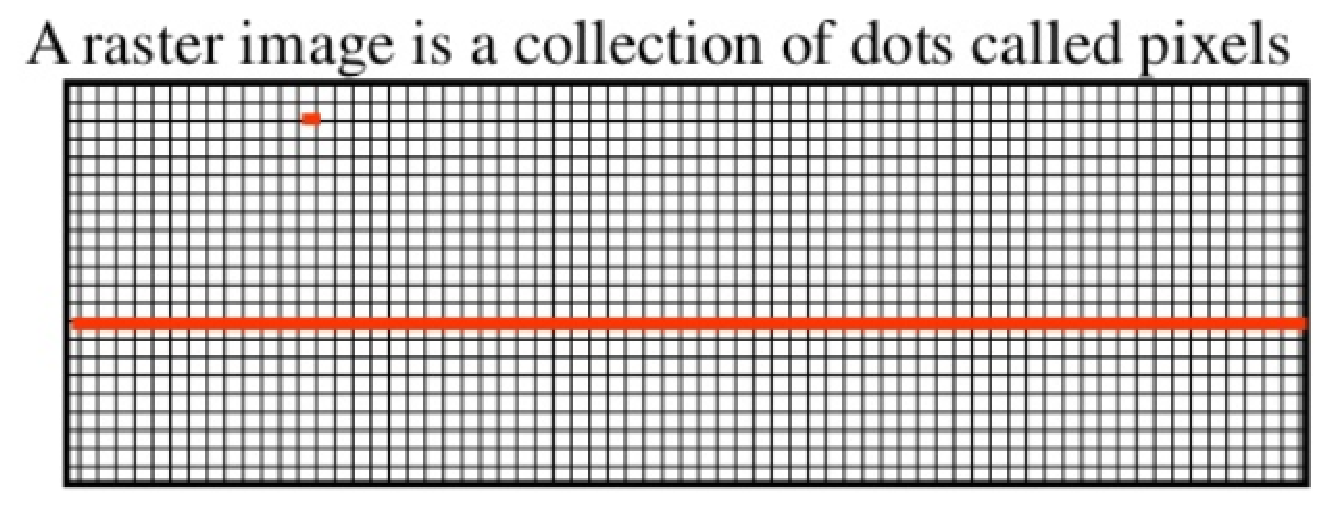
\includegraphics[height=5cm,
    angle=0]{./images/raster-display.eps}}
\caption{A raster display is a collection of dots called pixels}
\label{fig:raster-display}
\end{figure}

To draw a picture of a screen, we need the display controller
(Sect.\ref{sec:display-controller}) which draw the image stored in the memory
region (Sect.\ref{sec:frame-buffer}), following a certain refres procedure
(Sect.\ref{sec:refresh-procedure}).
  
\subsection{video controller (display controller)}
\label{sec:display-controller}

The display controller is a special processor, not the CPU, that control the
operation of the display device (Sect.\ref{sec:raster-screen}). 
This display controller read and process data from the frame buffer
(Sect.\ref{sec:frame-buffer}) and then can send image data to the terminal
display (e.g. printer, monitor, ..). If the terminal is the monitor
(Sect.\ref{sec:raster-screen}), the tracing beam following a given
strategy (Sect.\ref{sec:refresh-procedure}) to generate the exact content on
the screen.


To draw images to the terminal display, developers have to manually  convert RGB
color  values  into  the  current native screen format. Example: To  convert  an
RGB  value  to native  screen  format,  the  processor has  to  perform  up  to
ten operations  for  each  pixel  (four  AND,  three SHIFT  and  three  OR for
the  Palm  device). Since  this  is  a  costly  operation,  images  should  be
pre-rendered  to match  the  native  format  of  the  frame buffer   before  
being   used   in any   graphics   operations.
\begin{itemize}
  \item refreshing the screen
  
  \item transformation (e.g. enlarge a certain area, move a window)
  
\end{itemize}

% and  write  them  as
% bytes  to  the  frame  buffer  of the device (Sect.\ref{sec:frame-buffer}). This
% requires
% \begin{enumerate}
% 
%   \item cache  optimizations when  reading  and  writing  pixel  data  to  the  display  frame  buffer.
%   
%   \item   
% \end{enumerate}
% 


\subsection{refresh procedure}
\label{sec:refresh-procedure}

An image is divided into a sequence of (usually horizontal) strips known as {\bf
scan lines}, which can be further divided into discrete pixels for processing.
Each time the display controller (Sect.\ref{sec:display-controller}) needs to
update the screen, it controls the tracing beam following one of the below procedure
\begin{enumerate}
  \item  {\bf line by line}: the tracing beam scan from left to right, and then
  repeat to the next line. Lines start from first line, and once it reaches to the
  right most pixel on the last line, the tracing beam return to the left most of
  the first line.
  
This may cause flicker on raster display with slow refresh rate.
\begin{itemize}
  \item Horizontal retrace: (the electron beam follows horizontal tracing)
  refers to the return to the left (on next line) of the electron beam
  
  \item Vertical retrace: refers to the return to the top left corner of the
  electron beam
\end{itemize}

  
  \item {\bf interlacing}: there are two phases: even field and odd field.
   
   \item {\bf random-scan }: the electron beam directed to only the parts of
   the screen where a picture is to be drawn.
   
   It draws a picture one line at a time (vector display or stroke-writing or
   calligraphic display). So to draw a picture, the system goes through a set of
   commands in the {\bf display file} (display list), drawing each component
   line in turn.
 \begin{verbatim}
 Move 100,100
 Draw 200,140
 Text "hello!"
 Move 40,12
 ...
 
 Draw 100,1
 Jump start
 \end{verbatim}
   
   All components of a picture is drawn, i.e. refreshed, at a rate 30 to 60
   times per second.
   
   CONS: random-scan display only works well for line-drawing application; but
   not for realistic shaded scenes.
   
   
\end{enumerate}



\subsection{frame buffer: where picture is stored? (double buffer, triple
buffer, vsync)}
\label{sec:frame-buffer}
\label{sec:double-buffer-frame-buffer}
\label{sec:triple-buffer-frame-buffer}

When a computer needs to display something on a monitor, it draws a picture of
what the screen is supposed to look like and sends this picture (which we will
call a {\bf buffer}) out to the monitor.

\begin{itemize}
  \item  In the old days there was only one buffer and it was continually being
  both drawn to and sent to the monitor. 

ISSUE: when objects on the display were updated, they would often flicker.
  
  \item In order to combat the issues with reading from while drawing to the
  same buffer, {\it double buffering}, at a minimum, is employed.

The idea behind double buffering is that the computer only draws to one buffer
(called the "back" buffer) and sends the other buffer (called the "front"
buffer) to the screen. 

 After the computer finishes drawing the back buffer, the program doing the
drawing does something called a buffer "swap." This swap doesn't move anything:
swap only changes the names of the two buffers: the front buffer referencing
to the location of the back buffer and the back buffer referencing to the
memory location of the previous front buffer.

ISSUE: in this form of double buffering, a swap can happen anytime. That means
that while the computer is sending data to the monitor, the swap can occur. When
this happens, the rest of the screen is drawn according to what the new front
buffer contains. If the new front buffer is different enough from the old front
buffer, a visual artifact known as "tearing" can be seen. 
This type of problem can be seen often in high framerate FPS games when whipping
around a corner as fast as possible.  Because of the quick motion, every frame
is very different, when a swap happens during drawing the discrepancy is large
and can be distracting. 

  \item {\bf vsync}: Synchronizing buffer swaps with the Vertical refresh is
  called vsync.
  
Here, it waits to swap buffers until the monitor is ready for another image.
While enabling vsync does fix tearing, it also sets the internal framerate of
the game to, at most, the refresh rate of the monitor (typically 60Hz for most
LCD panels).

NOTE: With 60Hz, every frame takes just a little longer than 16.67 ms.

ISSUE: Input lag also becomes more of an issue with vsync enabled. This is
because the artificial delay introduced increases the difference between when something
 actually happened (when the frame was drawn) and when it gets displayed on
 screen.
 
NOTE: Input lag always exists (it is impossible to instantaneously draw what is
currently happening to the screen), but the trick is to minimize it.
  
   \item {\bf triple buffering}: it combines the best of both worlds with no
   sacrifice in quality or actual performance.
   
   
 There are 3 buffers: two back buffers, and one front buffer. This additional
 back buffer gives the computer enough space to keep a buffer locked while it is
 being sent to the monitor, i.e. if the new image is needed, it updates to the
 other back buffer, i.e. not affecting the buffer being sent to front buffer.
 Also, each time, the  front buffer is swapped for the back buffer containing
 the most recently completed fully rendered frame.
 
   \item {\bf flip-chain}:  multiple back buffers in a flip chain. A flip chain
   is simply two or more back buffers (sometimes called intermediary buffers)
   plus the primary surface (this is sometimes called triple-buffering,
   quadruple-buffering, etc.).   
   
 You have more than two back buffers. This is particularly useful when the
 amount of time spent drawing is greater than the monitor's refresh rate. 
 
In a flip chain, the next available back buffer becomes the primary surface,
 etc., all the way down to the rearmost back buffer that is used for drawing.
\end{itemize}
\url{https://docs.oracle.com/javase/tutorial/extra/fullscreen/doublebuf.html}

% Regardless of the type of image, i.e. raster or vector format, to be drawn
% (displayed) on a terminal, there must be a region where such information is
% stored. The picture definition (to be displayed on the monitor) is stored in a
% memory region called {\bf frame buffer} or {\bf refresh buffer}. 

Each terminal device has its own front framebuffer, that the display controller
(Sect.\ref{sec:display-controller}) understand and can read it.

Suppose the terminal is monitor, the information for each pixel, is called the
{\bf depth}, which can be
\begin{itemize}
  \item simply 1 bit per pixel (for black-and-white monitor). 

This frame buffer is called {\bf Bit map}.

  \item 16bits per pixel (i.e. 2 bytes/pixel)
  

  \item 24bits per pixel (typically holds RGB components, each with 8bits).
  
\end{itemize}
The order is also important: 
\begin{itemize}
  \item  Little Endian format: Palm O/S 5
  
  \item Big Endian: 
\end{itemize}

Basically, each location on the frame buffer holds the intensity values for the
associated pixel on the raster screen (Sect.\ref{sec:raster-screen}).
The pixel data in this frame buffer will be read in by the display controller
(Sect.\ref{sec:display-controller}), through a series of operations, before
painting a proper intensities on the monitor at the position associated with the
read-in pixel.

\subsection{frame buffer orientation}
\label{sec:frame-buffer-orientation}

For  design  reasons,  displays  are  internally  aligned  differently  on
various mobile devices, Fig.\ref{fig:framebuffer-orientation}. Form factor is
important, and the display and  its  connector  are  often  rotated  90  or  180
 degrees  to  decrease the physical size of the device. Currently there are
mobile devices available  with  all  of  the  four  possible  frame  buffer 
orientations.
\begin{itemize}
  \item \verb!xPitch! : numberof bytes need to add to move to the next pixel
  (on the same line)
  
  \item \verb!yPitch!: the number of bytes needed to add to move to the pixel on
  the next row.
\end{itemize}

\begin{figure}[hbt]
  \centerline{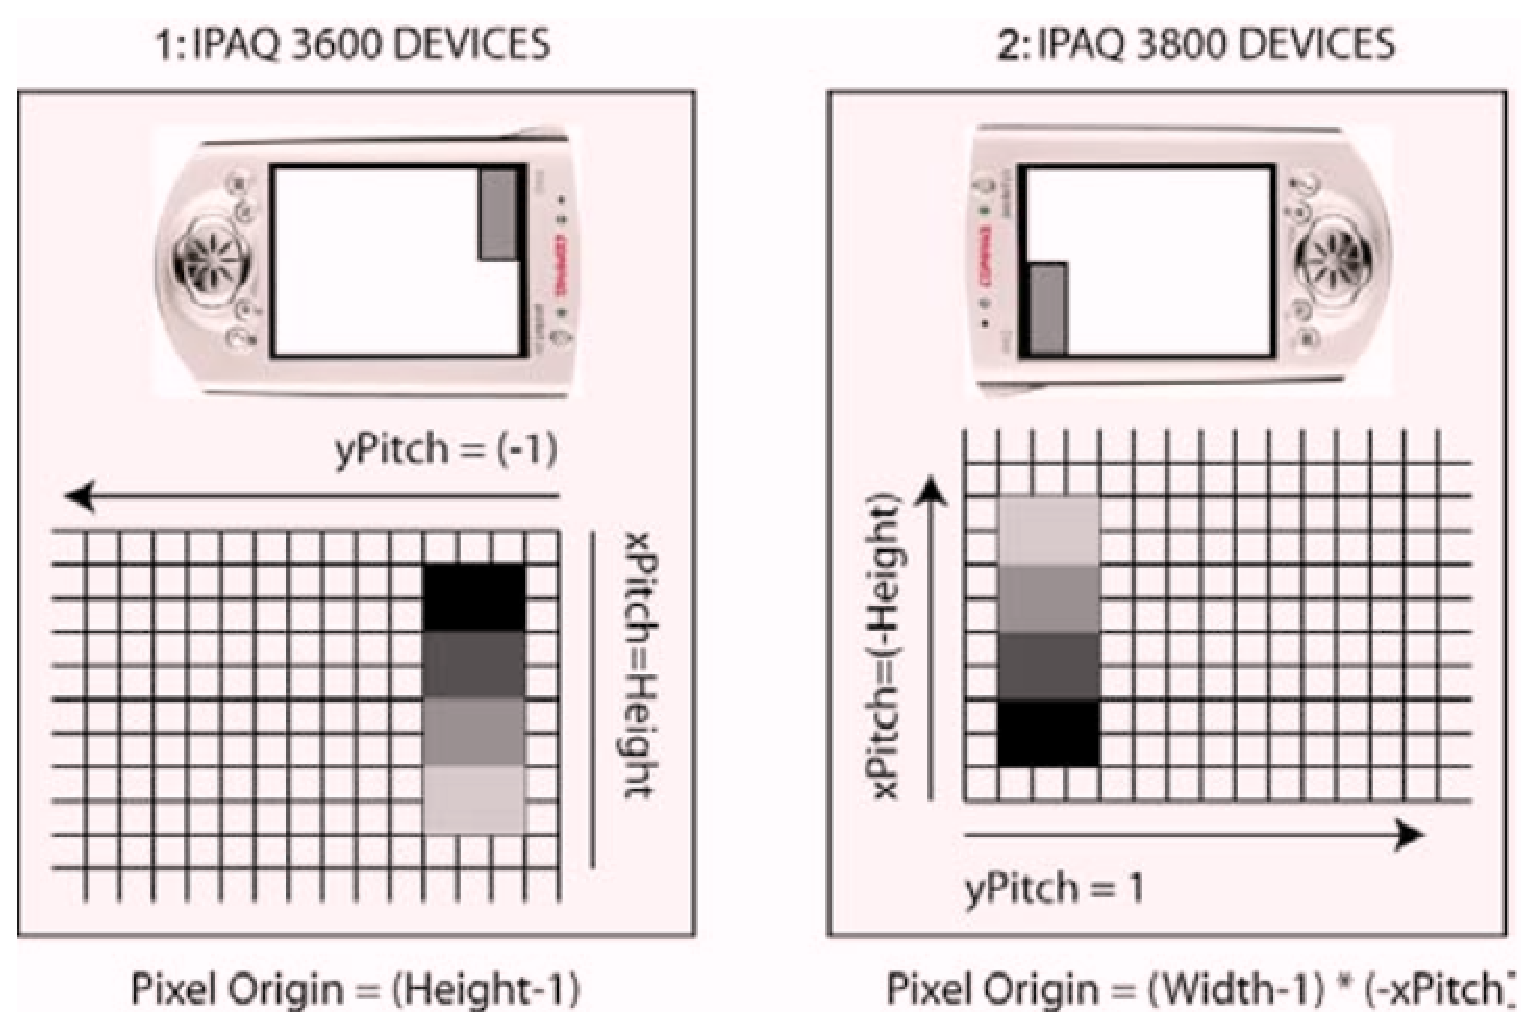
\includegraphics[height=5cm,
    angle=0]{./images/framebuffer-orientation.eps}}
\caption{Frame buffer orientation}
\label{fig:framebuffer-orientation}
\end{figure}

\subsection{Cache line and Data caches}

{\bf Cache line}: Reading  a  single  byte  from  any  location  in  memory 
will automatically  cause  a  computer  to  read  an  additional  number  of
consecutive  bytes  (a cache  line )  and  place  that  in  the  data  cache.
\begin{enumerate}
  \item ARM  CPU,  the  size  of  the  
cache line is 32 bytes

Reading  the  first  pixel  will  cause  the cache to automatically contain the
second, third, and up to the 32 nd pixel  of  that  same  row.

 \item 
\end{enumerate}
The {\bf data caches} stores a number of cache lines, i.e.
ARM  CPU  stores  256  cache  lines,  which  equals  
8kb  of  data  cache.

The  advantage  of  using  a  data  cache  is  that  data retrieved  from  the 
cache  is  accessed  significantly  faster  from  it than data from the main
system memory.




\section{History of widget toolkits}
\label{sec:history-widget-toolkits}

In early days of 1980s, it's not easy to create a GUI software that run on
different graphics hardware. The interface is not unique, i.e. it may looks
diffent when running on different hardware. Also, the manufacturers of the
graphics hardware need to develop the driver for each hardware.

X (Sect.\ref{sec:X11}) doesn't tell how the window or menu or button look like.
These are done by higher-level application software like 
\begin{enumerate}
\item window manager (e.g. twm, nautilus, ...)
\item GUI widget toolkit
\item desktop environment (e.g. KDE, GNOME, Windows...)
\end{enumerate}


\subsection{What is a widget?}
\label{sec:widget}

A widget, which is a combination of an X window and its associated input and
display semantics and which is dynamically allocated and contains state
information.

Widgets can be used
\begin{itemize}
  \item to display information (e.g. text or graphics) : textbox, \ldots
  
  \item as container for other widgets: e.g. menu box
  
  \item for output only and no interact with keyboard or cursor input :
  
  \item to response to input by invoking function that an application has attach
  to it.
\end{itemize}

Every widget belong to exactly one widget class. Logically, a widget class is
the procedures and data associated with all widgets belonging to that class.
Physically, a widget class is a pointer to a structure. The contents of this
structure are ``constant'' for all widgets of the widget class but will vary from
class to class. ``Constant'' means the class structure is initialized at compile
time and never changed, except for one-time class intialization of resource
lists when the first widget of the class is created.


\subsection{Xt}
\label{sec:Xt}

{\bf Xt} libray (Intrinsics) is the library developed on top of Xlib
(Sect.\ref{sec:Xlib}) with APIs to support the creating and using GUI components
starting from basic widgets (e.g. buttons, scrollbars) to complex (e.g. control
panels, property sheets), but still it has {\it no impose on the look and feel
of the widgets yet}.

These GUI components are collectively called {\bf widgets} -
Sect.\ref{sec:widget}. The libraries to provide the look-and-feel of these
widgets is described in Sect.\ref{sec:look_and_feel_specifications}.

Xt uses object-oriented programming techniques. This
allows extension to the list of available widgets by subclassing the existing or
writing a new wone based on the given conventions.
\begin{itemize}
  \item The root class is named {\bf Core} in the first version of Xt.
  
  \item Since Xt version 4, three non-widget superclasses are added above Core
  class, and the new root class is called {\bf Object}.
\end{itemize}
\url{http://www.x.org/docs/Xt/intrinsics.pdf}

Header files to use
\begin{verbatim}
// If using Intrinsic mechanism only
<X11/Intrinsic.h>
<X11/StringDefs.h>

<X11/Xatoms.h>
<X11/Shell.h>

// If want to implement widgets
<X11/IntrinsicP.h>
\end{verbatim}

\begin{mdframed}

On POSIX-based O/S, the Xt library is called \verb!libXt.a! and to link the
library we use \verb!-lXt!.
\end{mdframed}

\subsubsection{Core class}
\label{sec:Core_class}

The Core widget class contains the definitions of fields common to all widgets.


\subsection{Xaw (widget toolkit)}
\label{sec:Xaw}

Xaw (X Athena Widgets) is the GUI widget toolkit that built on top of Xt
library (Sect.\ref{sec:Xt}) as it imposes the look-and-feel of the different
widgets.

Depending on the widget to use, different header
files may also need to be included
\begin{verbatim}
<X11/Xaw/Label.h>

<X11/Xaw/Scrollbar.h>
\end{verbatim}

Xaw is maintained by X.org Foundation and is available as part of the X Window
System installation. 

However, Xaw has been largely superseded by more sophisticated toolkits like
Motif (Chap.\ref{chap:Motif}), GTK+ (Chap.\ref{chap:GTK+}), and Qt (Chap.\ref{chap:Qt}).  

\subsection{X toolkit (Xaw + Xt)}
\label{sec:X_toolkit}
 
Xt (Sect.\ref{sec:Xt}) and Xaw (Sect.\ref{sec:Xaw}) are collectively known as
the {\bf X Toolkit}.


\subsection{Motif}
\label{sec:Motif}

{\bf motif} is an industry standard toolkit/library for building GUI application
in X windows system since 1980s. Different implementations of the Motif API include Open
Motif, LessTif (Chap.\ref{chap:Motif}).  

\subsection{GLUI}
\label{sec:glui}

GLUI is a library with C++ interface, based on GLUT (Sect.\ref{sec:glut-2}), and
provides some user-control widgets (e.g. buttons, menu...). However, it doesn't
support advanced widgets like in Qt, wxWidgets or FLTK. 

% \subsubsection{FreeGLUT}
% \label{sec:freeglut-1}

% An alternate to GLUT, with some enhancements and less bugs. Read
% Sect.~\ref{chap:glut}


\section{Components in a widget toolkit}
\label{sec:UI-components-widget-tookit}

A UI element is aka a {\bf widget} or a {\bf control}.
A widget toolkit contains the implementation for a number of different classes.
Each class represent a UI element, such as textbox, menu, button, menuitem,
dialogbox, main window\ldots
These classes provides methods to interact with the control, or the data from
the control.

A GUI element is classified into one of the following groups
\begin{enumerate}
  \item GUI Component classes (such as Button, TextField, and Label) -
  Sect.\ref{sec:UI-Component}
  
  \item GUI Container classes (such as Frame, Panel, Dialog and ScrollPane) -
  Sect.\ref{sec:UI-Container}
   
  \item Layout managers (such as FlowLayout, BorderLayout and GridLayout) -
  Sect.\ref{sec:UI-Layout}
   
  \item Custom graphics classes (such as Graphics, Color and Font) - 
  Sect.\ref{sec:UI-custom-graphics-class}
 
\end{enumerate} 


When building a GUI application, we can either do it
\begin{itemize}
  \item programmatically : write the code to create the UI element using the
  above classes, identify its location, it's binding to which container
  
  
  \item drag-and-drop: with the help of GUI builders, you can quickly build a
  GUI application; the builder will generate the code for you, and you only need
  to write code to handle different events, i.e. the event handlers
\end{itemize}
\url{https://en.wikipedia.org/wiki/Widget_(GUI)}

Commercial libraries privdes (1) more UI elements; (2) some nice graphical
representations.

\subsection{Component classes}
\label{sec:UI-Component}

A Comonent class is a minimal class in a Widget Toolkit.

\subsection{-- Button}

There are subclases from Button:
\begin{enumerate}
  \item Radio Button
  
  \item Checked Box
  
  \item Split Button: 
  
  \item Cycle Button
\end{enumerate}

\subsection{-- Combo Box}

A combination of TextBox and an attached Menu or ListBox.
User can either enter the text or select the value from a drop-down list or
ListBox.

\subsection{-- Icon}


\subsection{-- Scrollbar}


\subsection{-- Slider}

control with a handle that can be moved up and down (vertical slider) or right
and left (horizontal slider) on a bar to select a value (or a range if two handles are present).

\subsection{-- List box}

\subsection{-- Spinner}

\subsection{-- Drop-down list}

\subsection{-- Menu}

\begin{enumerate}
  \item Context Menu
  
  \item Pie Menu
\end{enumerate}

\subsection{-- Menu Bar}

\subsection{-- Toolbar}

\begin{enumerate}
  \item Ribbon: an hybrid of menu and toolbar, displaying a large collection of
  commands in a visual layout through a tabbed interface.
\end{enumerate}


\subsection{Containers: group the widgets}
\label{sec:UI-Container}

A Container is used to group one or many Component object
(Sect.\ref{sec:UI-Component}) and/or one or many Container object
(Sect.\ref{sec:UI-Container})

Example:
\begin{enumerate}
  \item Window (aka Frame in some widget toolkits such as wxWidget)
  
  \begin{itemize}
    \item Model window
    \item Dialog Box
    \item Palette Window
    \item Frame (if the main window is Window)
    \item Canvas: a generic drawing element for representing graphical
    information.
  \end{itemize}
  
  
  \item panel
  
  \item tab
  
\end{enumerate}

\subsection{-- Window (Frame): Model window, Dialog box, Palette window,
Canvas, Applet}

\subsection{-- Panel}

\subsection{-- Tab}

\subsection{Custom graphics classes}
\label{sec:UI-custom-graphic-classes}

\subsection{-- Tree View}

\subsection{-- Grid View or DataGrid}

This is a complex widget what is as  a spreadsheet-like tabular view of data
that allows numbers or text to be entered in rows and columns.

\section{Look and Feel specifications}
\label{sec:look_and_feel_specifications}

While X Windows System (Sect.\ref{sec:X11}) is the de-facto standard for Unix
communication between client and server for graphical display, it does not
define the look and feel of the GUI. 

The development of look-and-feel tags along with the development of different
widget toolkits (Sect.\ref{sec:history-widget-toolkits}).

\subsection{OPEN LOOK}
\label{sec:OPEN_LOOK}

To help defining the standard for GUI look-and-feel, in Apr-1988, {\bf OPEN
LOOK} specification was created, a collaboration between Sun and AT\&T. The two
companies then formed OSF (Open Software Foundation) to manage OPEN LOOK.
OSF also created Motif GUI (Chap.\ref{chap:Motif}).

% The first O/S to have a look-and-feel is the Macintosh O/S, yet there is no
% standard in how the GUI components should look like.

OPEN LOOK: overall philosophy was to provide a clean, simple and uncluttered
interface, so that the user's focus would be on the application rather than the
interface. It is a definition of a look and feel rather than a specific
implementation
\begin{itemize}
  \item oval buttons, triangle glyphs: to indicate pull-down and pull-right menus
  
  \item "pushpins" which allowed the user to make dialog boxes and palettes stay visible. 
\end{itemize}


Widget toolkits that were developed using OPEN LOOK specification
\begin{enumerate}
  \item OLIT (OPEN LOOK Intrinsics Toolkit - introduced 1988): built on top of Xt (Sect.\ref{sec:Xt})
  \label{sec:OLIT}
    
  \item XView (introduced 1988): object-oriented API for C language. The source-code was pubclicly released in 1990.
  It is considered as the first open-source professional widget toolkit for X Window System.
  \label{sec:XView}
  
  UIT (User Interface Toolkit) is the C++ API to XView.
  
  XView was reputedly the first system to use right-button context menus, which is ubiquitously used.
  
\end{enumerate}

It is later abondoned in favor of Motif specificatioin (Sect.\ref{sec:Motif_specification})
and more recently GTK+ (Chap.\ref{chap:GTK+})

\subsection{Motif specification}
\label{sec:Motif_specification}

Motif user-interface specification is completely independent of how it is
implemented. So, you do not have to use the X Window System to implement a
Motif-style graphical user interface (GUI).

The first implementation of Motif specification use X Window System and X
Toolkit (Sect.\ref{sec:X_toolkit}) as the platform for the Application
Programmer's Interface (API), Xm library .

\url{http://www.ist.co.uk/motif/books/vol6A/ch-2.fm.html}

% Other widget sets:
% \begin{enumerate}
%   \item Athena widget set (Sect.\ref{sec:Xaw})
%   \item Motif (Chap.\ref{chap:Motif})
% %  \item OPEN LOOK (Sect.\ref{sec:OPEN_LOOK})
% \end{enumerate}


\subsection{Plugable look-and-feel}
\label{sec:look_and_feel_plugable}

Currently, only Swing widget Toolkit feature {\it plugable look-and-feel} - a
mechanism allowing users to change the look-and-feel of the program,
unrelated to the underlying platform.

The configuration file is XML, and can be changed at runtime.

\url{http://en.wikipedia.org/wiki/Pluggable_look_and_feel}


\section{Graphics Frameworks in Windows}

If you want to support Windows XP, using a "legacy" graphics framework is the
logical choice.

Starting at around Windows Vista, Microsoft has been
redesigning many of their API.
\begin{itemize}
  \item MMDevAPI: One True Sound API
  \item WIC: One True Image File API
  \item 
\end{itemize}
These new API's are much better than the old ones, and the "legacy" systems all
work based on the new ones.
Since Windows Vista and later, DirectSound is entirely based on MMDevAPI, and
components that need to read image files do it via WIC.

\subsection{'legacy' system (Windows XP): GDI, GDI+}
\label{sec:GDI}
\label{sec:GDI+}

The status designation of "obsolete" just means that the group responsible is no
longer accepting or fulfilling bug reports (except for critical security issues).

GDI isn't going anywhere, so if you need something rock-solid that is guaranteed
to be supported anywhere and everywhere, that's what I would go with.
If you need a bit more 2D capabilities than GDI offers (e.g., alpha channel
transparency), then you could consider using GDI+.

GDI+ is nearly an order of magnitude slower than GDI, but that's not too big of
an issue on modern machines with more power than you could ever want. This, too,
is going to be supported for a very long time to come.



\subsection{APIs on Windows RT}
\label{sec:GraphicsAPI_Windows-RT}

gdiplus, d3d9, and directdraw are present, but opengl is not.
 
 The only way to develop for Windows RT is through metro (now called the Windows
 8 Store), which restricts the old API's.

\section{Why no hardware-accelerated in 2D widget toolkits for mobile?}

Many features offered by the existing 2D APIs are difficult
or extremely expensive to implement using OpenGL. 

mobile GPUs are tile-based and aren't great in terms of raw pixel processing
power, but the pixel throughput would definitely be miles ahead of a general
purpose CPU.
I'm sure you guys have already considered this angle, but instead of using
OpenGL why couldn't you create a custom 2D graphics library for vendors to
implement at the lower level?

\url{https://groups.google.com/forum/#!topic/android-developers/D0PtrODTwBk}

However,  window composition is already hardware
accelerated and has been so since Android 1.0.

it really depends on what the application does exactly. If you
are always drawing the same translucent bitmap on screen, the GPU will
be better. If you are drawing complex shaded and antialiased paths or
you draw a bitmap that changes often, things can get pretty bad. Some
features of the Canvas API require other kinds of expensive operations
(for instance, implementing saveLayer/saveLayerAlpha requires the use
of FBOs or glCopyTexImage2D and neither solution is ideal.)


 Making a few fast paths for drawing bitmaps (BitBlt) would be huge for 
game developers.  I know that 3 of my games I have made aren't OGL 
simply because I don't want the extra code maintenance/burden.  If a 
game is doing some of the things you mention, well then it's not likely 
concerned with frame-rate.

Use OpenGL ES.


\section{Win32 GDI vs. Xlib}
\label{sec:WIN32_Xlib}

Win32 code using Win32 GDI (Sect.\ref{sec:Win32GDI}), while slightly opaque, is
miles easier to write then xlib code (Sect.\ref{sec:Xlib}). Xlib is miles more
complex then anything else, that is partially due to the fact that it was
developed to be a multi-client server.
\url{http://forums.anandtech.com/showthread.php?t=2054601}

A window created with native Win32 calls is about on the level of difficulty as
using the GTK+ to do the same thing. 

\begin{figure}[hbt]
  \centerline{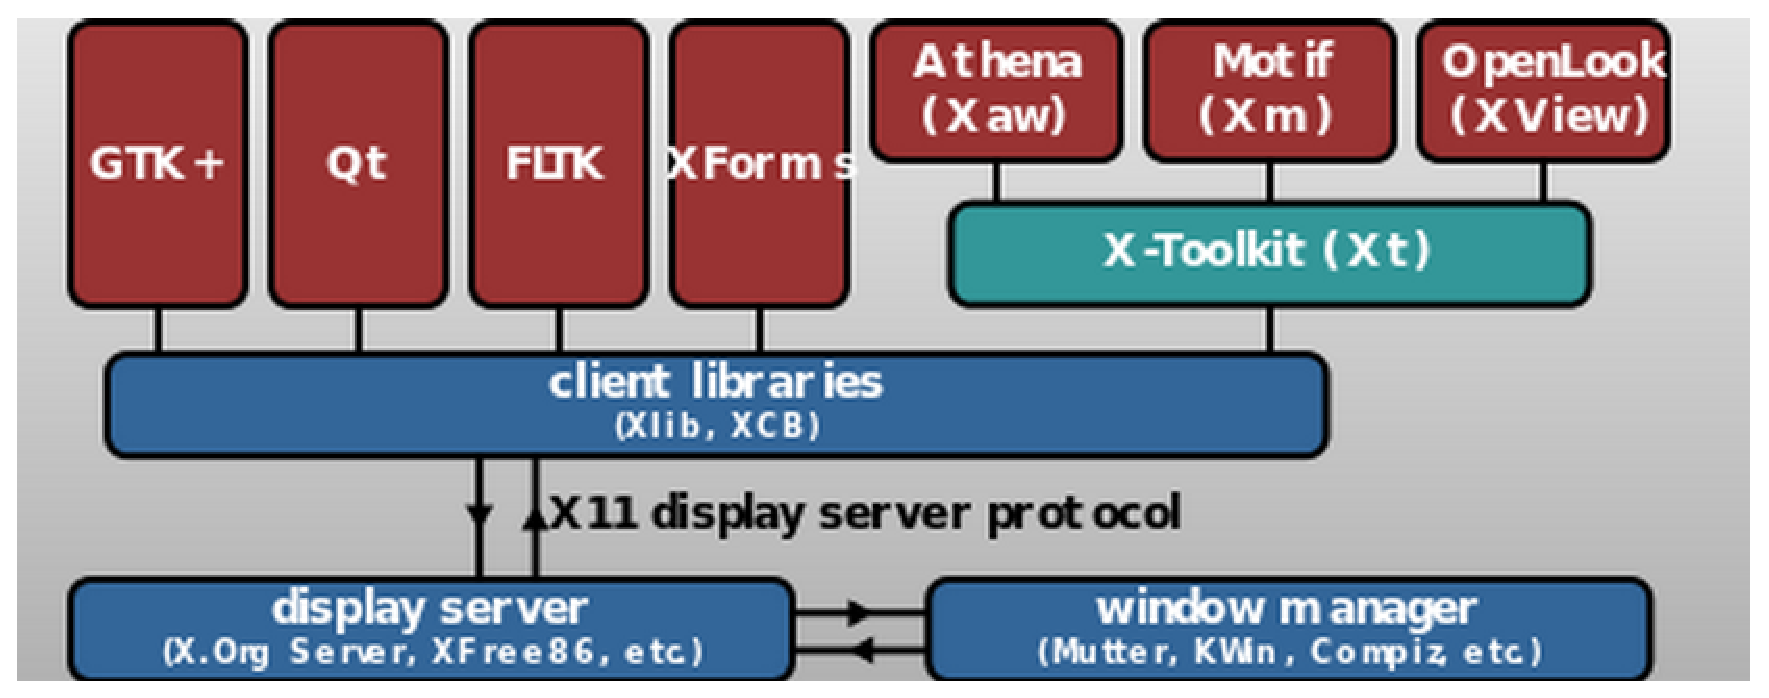
\includegraphics[height=5cm,
    angle=0]{./images/widget_library_system.eps}}
\caption{The hierachy structure of widget toolkits (X aw - Sect.\ref{sec:Xaw}, 
Xm - Sect.\ref{chap:Motif}, GTK+ - Sect.\ref{sec:GTK+},
Qt - Sect.\ref{sec:Qt}, FLTK - Sect.\ref{sec:FLTK}, XForms - Sect.\ref{sec:Forms_Library}),
XView - Sect.\ref{sec:XView}}
\label{fig:widget_library_system}
\end{figure}

\section{Widget Toolkits}
\label{sec:widget-toolkits-list}

A history is covered in Sect.\ref{sec:history-widget-toolkits}

\subsection{GUI Toolkits for C language}

\begin{enumerate}
  \item GTK - Chap.\ref{sec:GTK}
  \item Motif - Chap.\ref{chap:Motif}
  \item LessTif - Chap.\ref{chap:Motif}
\end{enumerate}

\subsection{GUI Toolkits for C++ language}

\begin{enumerate}
  \item GLUI - Sect.\ref{sec:glui}
  \item Qt - Chap.\ref{chap:Qt}
  \item Fox
  \item GTKmm - Sect.\ref{sec:GTKmm}
  \item FLTK - Sect.\ref{sec:FLTK}
  \item TCL/TK
  \item wxWidgets - Sect.\ref{sec:wxWidgets}
\end{enumerate}
\url{http://bwachter.lart.info/documentation/guitoolkits.html}

C++ in Windows
\begin{itemize}
  \item MFC (Sect.\ref{sec:MFC})
\end{itemize}

\subsection{GUI Toolkit for Python language}

\begin{enumerate}
  \item wxPython
  \item Tinker
  \item \ldots
\end{enumerate}
More information: Chap.\ref{chap:UI_Python}.

\subsection{GUI Toolkit for .NET languages (C\#)}

\begin{enumerate}
  \item WinForms: Sect.\ref{sec:Winform}
  \item WPF: from .NET 3.0
\end{enumerate}

\subsection{GUI Toolkits for Java}

\begin{enumerate}
  \item AWT
  \item Swing: more feature than AWT, native look-and-feel, and with the option
  of using a plugable look-and-feel defined by users (i.e. unrelated to
  the underlying platform) (Sect.\ref{sec:look_and_feel_plugable})
  
  
\end{enumerate}

\section{GUI builders}

GUI builders are software that help creating user interface easily (via using
drag-and-drop of mouse). The output is saved in some form of XML format (e.g.
XAML), and during the compilation, the builder will convert to source code of
the appropriate language and then regular compiler will compile to binary code.

\url{http://en.wikipedia.org/wiki/Graphical_user_interface_builder}


\section{Vector-graphics libraries}


\begin{enumerate}
  \item Cairo
\end{enumerate}

\section{Bitmap graphics libraries}

\begin{enumerate}
  \item ImageMagick
\end{enumerate}
\url{http://stackoverflow.com/questions/2650345/imagemagick-vs-cairo-on-vector-graphics-rasterization}

\section{Design Languages}

Design language (design vocabulary) refers to a style that guides the design of
a complements of products to give a consistent look and feel. There are
different choices: materials, colour schemes, shapes, patterns, textures, or
layouts. 

In automobiles, the design language is often in the grille design.
In software architecture, design languages are related to architecture
description languages. The most well-known design language is UML. Others design
language in software
\begin{enumerate}
  \item Material Design (Sect.\ref{sec:MaterialDesign})
  \item Microsoft Metro design language (Sect.\ref{sec:Microsoft_Metro})
  \item Snow White design language (Sect.\ref{sec:SnowWhite})
\end{enumerate}

\subsection{Microsoft Metro}
\label{sec:Microsoft_Metro}

{\bf Metro} is a typography-based design language. The key design is focusing on
the content of applications, relying more on typography (emphasizes
cleanliness, readability and objectivity) rather than the graphics. 

Metro is being used in Windows 8. Early response to the language was generally
positive, but become negative with Windows 8 as it's frustrating and various
aspects of the UI did not work well together. Also, full-screens apps are being
used as thus Microsoft has shift the focus away from multi-tasking and business
productivity.

\subsection{Snow White}
\label{sec:SnowWhite}

The scheme has vertical and horizontal stripes for decoration and it is being
used in many Apple computer from 1984 to 1990. This is for hardware, but not for
software.
\url{http://en.wikipedia.org/wiki/Snow_White_design_language}

\subsection{Material Design}
\label{sec:MaterialDesign}

{\bf Material Design} is a cleaner design that uses grid-based layouts,
with a lot of responsive animations and transitions, padding and depth effects
(e.g. lighting and shadows). Every time we press, there is always a responsive
animation effect. Material Design is built around the idea of
treating the virtual space within your smartphone as if it were a physical object. "What if pixels
didn't just have color, but also depth?" said Google's VP of Design Matias
Duarte.
\footnote{\url{http://www.npr.org/blogs/alltechconsidered/2014/11/16/364152727/googles-lollipop-wants-to-change-the-way-we-use-our-phones}}
\url{http://android-developers.blogspot.com/2014/10/implementing-material-design-in-your.html}

Material Design is used in Android 5.0 (Lollipop). The API for third-party
development to incorporate the design into their applications is 
\url{http://www.google.com/design/spec/material-design/introduction.html}

\url{http://bgr.com/2014/07/30/google-drive-material-design-update/}

It shoulds provide a consistent UI for different platform and device sizes. 
Mobile precepts are fundamental, but touch, voice, mouse, and keyboard are all
first-class input methods.

In material design, UIs are composed of pieces of digital paper \& ink. 
The surfaces and the shadows they cast provide visual cues to the structure of
the application, what you can touch and how it will move. This digital material can move, expand and reform to create flexible UIs.

A material is based on the concept of paper and the content is just like ink
(adding no additional thickness). A material environemt is a 3D space (with
x,y,z dimensions). The z-axis aligns with the plane of the display, with
positive z-axis extending towards the viewer. So, every sheet of material
occupies a single position along the z-axis with a standard 1.0dp thickness; and
with different x- and y- dimentions. Content does not add thickness to material.

Depending on the direction of the virtual light source, a material can cast
shadow on another one. There are two types of light sources:
\begin{itemize}
  \item key light : the first and usually the most important light that a
  photographer (cinematographer, lighting camerman, \ldots) uses in a lighting
  setup.
  \url{http://en.wikipedia.org/wiki/Key_light}
  
  \item ambient light : usually refers to sources of light that are already
  available naturally, not explicitly supplied by the photographer for the
  purpose of taking the photos
\end{itemize}
A key light creates directional shadows, while an ambient light creates
consistent, soft shadows from all angles.
All shadows in the material environment are cast by these two light sources.
Shadows are the absence of light resulting from the occlusion of these light
sources by sheets of material at various positions along the z-axis.

Content behavior can be decoupled from the behavior of material. However, the
bounds of the material can limit the display of the content. It means that if
the material is rezied, the content keep unchanged until we resize the content. 


Material cannot pass through other material. For example, one sheet of material
cannot pass through another sheet of material when changing elevation. This maps
exactly the same in real-world. In the physical world, objects can be stacked or
affixed to one another, but cannot pass through one another

Transforming material
\begin{enumerate}
  \item change shape
  \item grow/shrink along only its plane
  \item never bends or folds (i.e. always on a single z-plane)
  \item Sheets of material can join together to become a single sheet of
  material.
  \item When split, material can heal. For example, if you remove a portion of
  material from a sheet of material, the sheet of material will become a whole sheet again.
  \item can move along any axis.
  
  Z-axis motion is typically a result of user interaction with material.
  Elevation is the relative value between parent and child objects.
  Elevation is measured in the same units as the x and y axes, typically in
  density independent pixels (dps). Since material has a standard 1dp thickness,
  all elevation distances are measured from one top surface to another top surface. 
  
  All material objects have a resting elevation, whether the object is a small
  component or a sheet that spans the entire display. If an object changes
  elevation, it should return to its resting elevation as soon as possible.
  The resting elevation for a given UI component type is consistent across apps
  throughout a platform. However, that same component type may have different
  resting elevations from platform to platform depending on the depth of the
  environment (e.g., TV has a greater depth than mobile or desktop).  
  
  \item Material can be spontaneously generated or destroyed anywhere in the
  environment.
\end{enumerate}

Objects can move independently of each other, or their movement can be
constrained to, and dependent upon, their container. Containers and the objects
they contain have a parent-child relationship. Every object has a single parent,
and may or may not have one or more children.  

\section{VCL (Visual Component Library)}
\label{sec:VCL}

VCL is the visual component-based object-oriented framework, written in Object
Pascal, and is used to develop GUI for Windows applications.
VCL forms a class hierarchy with a common ancestor, i.e. the root base-class
\verb!TComponent! class which inherits from the root class \verb!TObject! in
Delphi Object Pascal. This is utilized in Java, Smalltalk, C\#, etc.
\begin{itemize}
  \item TForm class: windows
  \item TButton, TCheckBox, TLabel classes: controls
  \item database access: 
  \item Internet connections: 
\end{itemize}

VCL supports multithreading, even though not all VCL components are thread-safe. 

\section{.NET}

.NET is good for

\section{Winform}
\label{sec:Winform}

Winform is very much easy. Much of its design is based on VCL
(Sect.\ref{sec:VCL}).

More details: Chap.\ref{chap:Windows.Forms}

Application that use: TortoiseSVN

\section{Qt}
\label{sec:Qt}

Qt used a thing called {\bf MOC} (Meta Object Compiler) which was designed for reflection. 
Qt invented the signal and slot system using in Boost and GTK. Thus, Qt is an event-based GUI framework.

When a user clicks a button it'd send a message (signal) and whatever slot was
connected to the signal would get that event and respond however to it. It is
type safe, you don't have to worry about it messing up. It will just not call
the invalid slot and will report the error letting you know.


Qt has a designer application {\bf Qt-Creator} that allows you to create signals
in it, wide range of widgets to use.
You can even make a widget plugin and put your own widgets in to designer and
drag them on to the form and see it in real time.
You can see the code it generates (via MOC) and spits out 100\% valid C++.

Qt ships with a lot of modules in it. Ranging from SQL, network, XML,
XSLT/XPath, to WebKit. Even COM support (which only runs on Windows).

 QtActive, you can make Qt plugins for Internet Explorer if you want
 
  QtScript, which allows you to add scripting to your application via JavaScript if you would like to have i


  
\section{UI Data binding}
\label{sec:data-binding-UI}


{\bf UI data binding}
\footnote{\url{http://en.wikipedia.org/wiki/UI_data_binding}} is a software
design pattern to simplify the development of GUI application. Each UI element
can bind to an application domain model
(Sect.\ref{sec:software-dev-practices}), Fig.\ref{fig:UI-databinding}.
\footnote{\url{http://msdn.microsoft.com/en-us/library/wxt2cwcc.aspx}}

Once there is a change in the datasource, the UI controls on the GUI form should
be able to get updated. The datasource can be the traditional data sources (e.g.
relational database) or can come in the form of any structures that contains
data (e.g. databases, web services, and objects). Depending on the GUI packages
(e.g. WinForms, WPF, Unity, \ldots), different UI data binding techniques are
supported.


\begin{figure}[hbt]
  \centerline{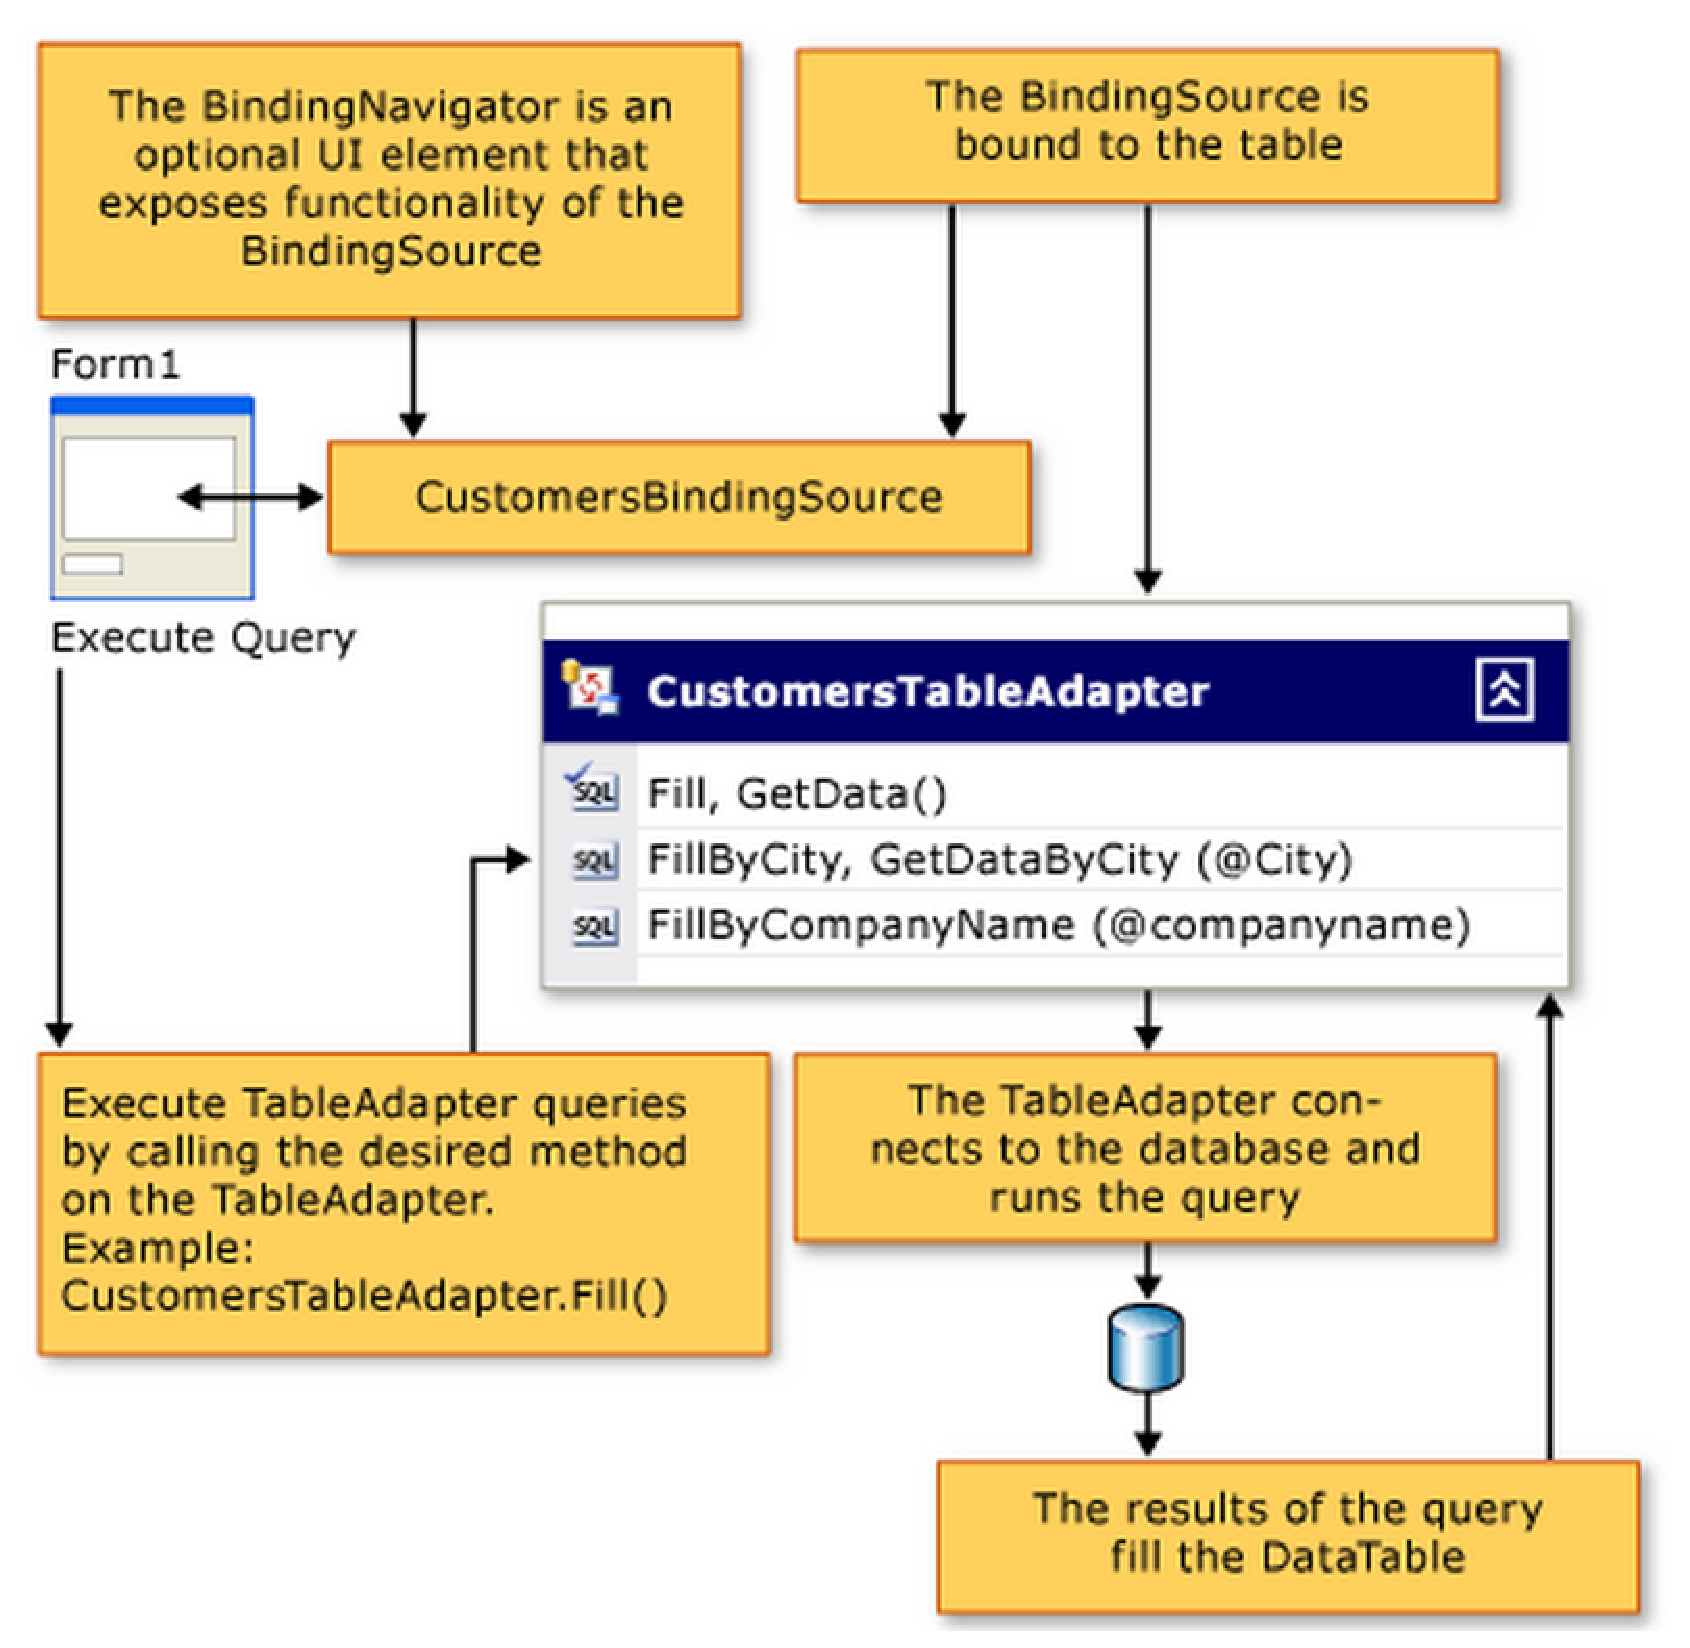
\includegraphics[height=5cm,
    angle=0]{./images/UI-databinding.eps}}
  \caption{UI-databinding}
\label{fig:UI-databinding}
\end{figure}


\section{Software Development Practices}
\label{sec:software-dev-practices}


In UML, a class diagram is used to represent a {\bf Domain
Model}\footnote{\url{http://en.wikipedia.org/wiki/Domain_model}}.
The Domain Model is one of the central parts in FDD (Sect.\ref{sec:FDD}).

\subsection{FDD (Feature-Driven Development)}
\label{sec:FDD}

FDD emphasizes on the progress made for each feature. A feature is a relatively
small task. FDD defines 6 milestones per feature that are to be completed
sequentially. The first 3 are completed during {\bf Design by Feature} activity;
and the last 3 are done during {\bf Build by Feature} activity.
\footnote{\url{http://en.wikipedia.org/wiki/Feature-driven_development}}

Each milestone has a percentable complete value assigned to help tracking the
progress. Example: a feature still being coded with 44\% complete can have
(Domain Walkthrough 1\%, Design 40\% and Design Inspection 3\% = 44\%).

\begin{enumerate}
  \item {\bf Domain Object Modeling}: after explore and explain the domain of
  the problem to be solved; this provdies an overall framework in which new
  features can be added.
  
  \item {\bf Developing by Feature}: any function too complex to be implemented
  within 2 weeks is further decomposed into smaller functions until each
  sub-problem is small enough to be called a {\it feature}. 
  
  Features in this respect were small pieces of client-valued functions
  expressed in the form \verb!<action> <result> <object>!, for example:
  'Calculate the total of a sale' or 'Validate the password of a user'.
  
  This makes it easier to deliver a correct function and to extend/modify the
  system. After the feature list had been completed, the next step was to
  produce the development plan. 
  
  \item {\bf Individual Class (code) Ownership}: distinct pieces or grouping of
  codes are assigned to a single owner. The owner is responsible for the
  consistency, performance, and conceptual integrity of the class.
  
  Class ownership has been done by ordering and assigning features (or feature
  sets) as classes to chief programmers.
  
  \item {\bf Design by Feature}: 
  the chief programmer worked out detailed sequence diagrams for each feature
  and refines the overall model. Next, the class and method prologues are written and finally a design inspection is held.
  
  \item {\bf Buid by Feature}: After a successful design inspection a per
  feature activity to produce a completed client-valued function (feature) is
  being produced. The class owners develop the actual code for their classes. 
  
  
  After a unit test and a successful code inspection, the completed feature is
   promoted to the main build.
  
  
\end{enumerate}

\section{FLTK (Fast Light Toolkit)}
\label{sec:FLTK}

FLTK (``fulltick'') is a light-weight cross-platform GUI toolkit for
UNIX/Linux(X11)/Windows/MacOS X. It was designed to be compatible with
{\bf Forms Library} (Sect.\ref{sec:Forms_Library}). So all functions of FLTK are
also prefixed with \verb!fl_!. 

FLTK is LGPLv2 licensed, with exception ``allow for static linking''. 

FLTK was designed to be statically linked. It is also designed so that all data
used by the GUI, such as images and widget layout, can be inlined into source code.


A GUI Design IDE for FLTK is called FLUID (Fast Light User Interface Designer).
The FLUID program (which includes every widget) is only 352k. 
The output of FLUID is a \verb!*.fl! file and can also be converted to C++
source code and header file.
\url{http://www.fltk.org/documentation.php/doc-1.1/fluid.html}

\subsection{version}

FLTK 1.3:
\begin{verbatim}
svn co http://seriss.com/public/fltk/fltk/branches/branch-1.3/ fltk-1.3

cd fltk-1.3 
// to update
svn update
\end{verbatim}


\subsection{compile fltk in Ubuntu 16.04 on Debian 8 (i.e. Ubuntu 14.04)}
\label{sec:fltk-1.3+-Ubuntu-14.04}

\begin{verbatim}
sudo apt-get build-dep -y libfltk1.3
sudo apt install -y cmake

$ mkdir fltk
$ cd fltk
$ URL=http://archive.ubuntu.com/ubuntu/pool/universe/f/
$ wget ${URL}/fltk1.3/fltk1.3_1.3.3.orig.tar.gz
$ wget ${URL}/fltk1.3/fltk1.3_1.3.3-8.dsc
$ wget ${URL}/fltk1.3/fltk1.3_1.3.3-8.debian.tar.xz
$ tar zxvf fltk1.3_1.3.3.orig.tar.gz
$ cd fltk-1.3.3/
$ tar xvf ../fltk1.3_1.3.3-8.debian.tar.xz

//build
dpkg-buildpackage -us -uc

//now we can install
$ cd ..
$ sudo dpkg -i *.deb || (sudo apt -f install -y ; sudo dpkg -i *.deb)
$ cd ..
\end{verbatim}



\subsection{compile fltk from source}
\label{sec:fltk-compile}

NOTE: FLTK 1.3+ requires libpng 1.4+ (Sect.\ref{sec:libpng}), as it uses
\begin{verbatim}
The "png_set_longjmp_fn()" API was introduced in libpng-1.4.x. Ubuntu 13:10
currently comes with libpng-1.2.49 (see /usr/include/libpng12), which does not
supply png_set_longjmp_fn(). 
\end{verbatim}
\url{https://stackoverflow.com/questions/21545076/libpng-png-set-longjmp-fn-not-found}

We need to update \verb!CMAKE_CXX_FLAGS! to get proper link to the library
\begin{verbatim}
rm * -rf ; cmake -DCMAKE_INSTALL_PREFIX:PATH=/packages/fltk/1.3/
 -DCMAKE_PREFIX_PATH=/packages/libpng/1.5 -DCMAKE_REQUIRED_LIBRARIES=-lpng
 -DCMAKE_REQUIRED_INCLUDES=/packages/libpng/1.5/include
 -DCMAKE_CXX_FLAGS="-I/packages/libpng/1.5/include -L/packages/libpng/1.5/lib -lpng" \
 ../; make -j4 
\end{verbatim}

If the fltk library is installed via Cmake, it will create these files
\begin{verbatim}
/packages/fltk/1.3/share/fltk/FLTK-Functions.cmake
/packages/fltk/1.3/share/fltk/FLTK-Targets-noconfig.cmake
/packages/fltk/1.3/share/fltk/FLTKConfig.cmake
/packages/fltk/1.3/share/fltk/UseFLTK.cmake
/packages/fltk/1.3/share/fltk/FLTK-Targets.cmake
\end{verbatim}

\subsection{writing GUI using FLTK}

IMPORTANT:
\begin{verbatim}
#include <fltk/Window.h>
#include <fltk/Widget.h>
#include <fltk/run.h>
using namespace fltk;
\end{verbatim}

Then, we create a window of class \verb!Window!, add as many widgets as you
want, and show the window
\begin{verbatim}
int main(int argc, char **argv) {
  Window *window = new Window(300, 180);
  window->begin();
  Widget *box = new Widget(20, 40, 260, 100, "Hello, World!");
  box->box(UP_BOX);
  box->labelfont(HELVETICA_BOLD_ITALIC);
  box->labelsize(36);
  box->labeltype(SHADOW_LABEL);
  window->end();
  window->show(argc, argv);
  return run();
}
\end{verbatim}

To compile your code
\begin{verbatim}
g++ `fltk-config --cxxflags` snippet.cpp `fltk-config --libs` -lX11 -ldl -lXext
-lXinerama -lXft -lfontconfig -o snippet
\end{verbatim}
NOTE: \verb!fltk-config! (with the flag \verb!--libs! for linker, and
\verb!--cxxflags! for header file) can be used to produce a set of flags to pass
to your gcc.


\section{Forms Library and XForms}
\label{sec:Forms_Library}

Forms Library is written for SGI machines. Its derivative is XForms

In Forms Library, all functions are prefixed with \verb!fl_!.


\section{MFC}
\label{sec:MFC}

MFC is thinnest layer over Win32, GUI, controls, DLL, file IO, multithreading etc.
It is thin layer over socket, networking, internet programming.
And it facilitates COM programming with thickest layer.

MFC use {\bf message maps} (Sect.\ref{sec:message_map}) as an alternative to the
switch statement used in traditional Windows programs to handle messages sent to
a window.

\url{https://wiki.wxwidgets.org/WxWidgets_Compared_To_Other_Toolkits}

\subsection{message map}
\label{sec:message_map}

Message Maps maps the user action into the appropriate MFC class functions to handle it. 
A mapping from messages to member-functions may be defined so that when a
message is to be handled by a window, the appropriate member function is called
automatically.

The advantage of Message Map is the same action can be mapped to more than one
MFC class function.
This message-map facility is designed to be similar to virtual functions but has
additional benefits not possible with C++ virtual functions.

The MFC Class which can handle message should be member of CCmdTarget, (i.e.) it
should be hierarchically derived from CCmdTarget.

To do the mapping, MFC define a macro \verb!DECLARE_MESSAGE_MAP!. A Class wizard can help you to create a class
\begin{verbatim}
class CMyWnd : public CMyParentWndClass
{
    // my stuff...

protected:
    //{{AFX_MSG(CMyWnd)
    afx_msg void OnPaint();
    //}}AFX_MSG

    DECLARE_MESSAGE_MAP()
};
\end{verbatim}
that automatically add \verb!//{{! and \verb!//}}! brackets.

\url{https://msdn.microsoft.com/en-us/library/aa267978.aspx}


\section{Event-driven app}
\label{sec:event_driven_app}

In an event-driven application, there is generally a main loop that listens for
events, and then triggers a callback function when one of those events is
detected. Event-driven programming is widely used in GUI apps.

\begin{mdframed}
In embedded systems the same may be achieved using hardware interrupts instead
of a constantly running main loop.
\end{mdframed}


The first step in developing an event-driven program is to write a series of
subroutines, or methods, called event-handler routines (or {\it callback
function} - a term in Windows).

\url{http://en.wikipedia.org/wiki/Event-driven_programming}


\section{DirectX}
\label{sec:DirectX}

Microsoft DirectX is a collection of APIs for handling
tasks related to multimedia, especially game programming and video, on
Microsoft platforms.
Originally, they are separated libraries: 
Direct3D, DirectDraw, DirectMusic, DirectPlay, DirectSound, \ldots
The name DirectX was coined as shorthand term for all of these APIs.

DirectX 1.0 is the replacement for WinG APIs (Sect.\ref{sec:WinG}) when
switching from Windows 3.1 to Windows 95. Like WinG, DirectX 1.0 was designed to
enable direct access to hardware devices (video cards, keyboards, mice, sound
devices).
\begin{itemize}
  \item DirectX 8.0 is the last version to have software rendering support.

  \item DirectX 9.0c RC0 is the first to have 64-bit capable build.
\end{itemize}

DirectX includes APIs not only for GUI, but also for multimedia processing
(DirectMusic, DirectPlay, DirectSound).
Here we introduce APis for GUI
\begin{enumerate}
  \item DirectDraw : until DirectX 8.0, then merged into Direct3D
  \item Direct3D: added since DirectX 3.0 version number 4.04.00.0069
  
Direct3D (Sect.\ref{sec:Direct3D}) however, focused on game use.  
\end{enumerate}

\section{Java-based libraries}

native rendering libraries with Java APIs 
\begin{enumerate}
  \item Mophun
  by  Synergenix,  
  
  \item Brew
  by  Qualcomm  and
  
  \item JBlend by  Aplix
\end{enumerate}

Typically,  Java-Based  Graphic  APIs  such  as  
Brew  or  JBlend  only  work  on  mobile  phones,  making  it  difficult  
to target other devices such as handheld computers using the same 
code  base.



\section{Desktop Environment}
\label{sec:desktop_environment}

\begin{verbatim}
>> echo $DESKTOP_SESSION

gnome


>> ps -ef | grep gnome

>> ps -A | egrep -i "gnome|kde|mate|cinnamon|lxde|xfce|jwm"
\end{verbatim}

\subsection{GNOME}

Sect.\ref{sec:GNOME} in 'GUI development' book discusses in depth.

GNOME2 used Metacity window manager (Sect.\ref{sec:Metacity}).

GNOME3 used Mutter window manager (Sect.\ref{sec:Mutter}). 

\subsection{Unity}
\label{sec:Unity}

Unity was first developed by Canonical to replace GNOME 2. However, after 7
years, Canonical now switched back to GNOME 3 in Ubuntu 18.04.

It has a bar at the top which contains the clock at the right and a button on
the left which will bring up a search/menu window. There's a launcher on the
left of the screen. The default theme color is purple/orange/brown.

\subsection{MATE}
\label{sec:MATE}

MATE is a fork of Gnome 2. It features two bars, one on the top of the screen,
one at the bottom. 
\begin{enumerate}
  \item  The top one contains the main menu (dropdown with three items,
  Applications, Places and System), some starters and the clock on the far right. 
  
  \item The lower bar holds the window list and the desktop switcher.
\end{enumerate}
MATE also has icons (Computer, Home, Trash and also removable media) on the
desktop in the default configuration.

\subsection{XFCE}
\label{sec:XCFE}

XFCE is very similar to MATE/Gnome 2 and might easily be confused with the two.
The default configuration is similar to MATE/Gnome 2 except that the menu in the
upper bar is only an icon, but is similarly structured.

\subsection{KDE}
\label{sec:KDE}

KDE is one of the oldest desktop environments. It features a bar at the bottom
of the screen which contains the main menu (as icon), the window list and a
clock. The main menu is a big dropup menu sorted in categories. 

\subsection{Cinnamon}
\label{sec:Cinnamon}

Cinnamon is heavily based on Gnome 3. It features a lower bar similar to KDE, as
it contains the menu button, the window list and the clock.




\section{Window Manager}
\label{sec:window_manager}

\url{http://en.wikipedia.org/wiki/Comparison_of_X_window_managers}

To ensure different window managers provide a consistent interface for the
applications to interact, a window manager should be designed following NetWM
(or EWMH - {\it Extended Window Manager Hints}) standards
\url{http://blackboxwm.sourceforge.net/NetWM}.
The older version of NetWM is called ICCCM (Inter-Client Communications
Conventions Manual) - Sect.\ref{sec:ICCCM}.

\subsection{ICCCM}
\label{sec:ICCCM}
\label{sec:selections}
\url{https://tronche.com/gui/x/icccm/}

\begin{mdframed}
In X10, "cut buffers" were introduced. These were limited buffers that stored
arbitrary text and were used by most applications.  Cut buffers are long
deprecated, and although some applications (such as xterm) may have legacy
support for them, it is both not likely and not recommended that they be used.  

In the old "cut buffers" system where arbitrary applications could modify data
stored in the cut buffers. In ICCM, only one application may control or "own" a
selection at one time. So, when that application is closed, the selection text
is lost.
\end{mdframed}

\begin{itemize}
  \item ICCM version 2.0  is standardized in X11R6 (Sect.\ref{sec:X11R6})
\end{itemize}

{\bf Selections} are the primary mechanism that X Version 11 defines for the
exchange of information between clients, for example, by cutting and pasting
between windows.

There can be an arbitrary number of selections (each named by an atom) and that
they are global to the server. 
\url{https://tronche.com/gui/x/icccm/sec-2.html}

To conform with the inter-client conventions, however, clients need deal with
only these three selections, named by the atom  
\begin{enumerate}
  \item PRIMARY
  
  used by the commands that take only a single argument and is the principal
  means of communication between clients that use the selection mechanism. 
  
  \item SECONDARY
  
  used as (1) the second argument to commands taking two arguments; 
  (2)  a means of obtaining data when there is a primary selection and the user
  does not want to disturb it 
  \item CLIPBOARD
  
  used to hold data that is being transferred between clients, that is, data
  that usually is being cut or copied, and then pasted
\end{enumerate}
respectively.\footnote{\url{https://tronche.com/gui/x/icccm/sec-2.html\#s-2.6}}

Of the three selections, users should only be concerned with PRIMARY and
CLIPBOARD.   
\begin{itemize}
  
  \item The CLIPBOARD selection is accessed using keyboard shortcuts, while
application specific, these are most commonly ctrl+c for copying, ctrl+v for
pasting and ctlr+x for cutting.

The clipboard may also contain other items than text, such as images or folders.

  \item  The PRIMARY selection speeds up the copying task by copying the text to
  the clipboard as soon as it was selected with the mouse, without the need for
  entering a keyboard shortcut.  
  
   Pasting is triggered by pressing the middle mouse button (or some emulation
   of it). 
\end{itemize}
\url{https://wiki.archlinux.org/index.php/Clipboard\#List_of_clipboard_managers}

Other selections may be used freely for private communication among related
groups of clients. 

Let's discuss some application's behavior with the PRIMARY selection and
CLIPBOARD selection
\begin{enumerate}
  \item gvim with \verb!+clipboard! feature
  
  \verb!*! register represents the PRIMARY buffer in X.
  
  vim's command \verb!:yank! (or yank selected text with yy; or yank current
  work with yw; or yank current character with yc) and \verb!:paste! 
 operate on unnamed register, which by default corresponds to \verb!*! register.
 
  
  \item the list of clipboard managers
  
\begin{verbatim}
Xclip - A lightweight, command-line based interface to the clipboard.

Autocutsel - Command line and daemon interfaces to synchronize 
             PRIMARY, CLIPBOARD and cut buffer selections.
 
\end{verbatim}
  \url{https://wiki.archlinux.org/index.php/Clipboard\#List_of_clipboard_managers}
\end{enumerate}



\subsection{Blackbox}

Blackbox is the fast, lightweight window manager for the X Window System
(version 6+).
lackbox is built with C++ and contains completely original code (even though the
graphics implementation is similar to that of WindowMaker or NeXT interface).
\begin{itemize}
  \item The first stable Blackbox release (0.51.3.1) was built from only 14,406
  lines of code (includes source, headers, comments and preprocessor
  statements). The latest version has around 40,000 lines. 
  
\end{itemize}

Blackbox itself does not directly handle key bindings like  most  other
window  managers.  This  task  is  handled by a separate utility called
\verb!bbkeys!.
The slit is an edge of the screen which  can  hold  specially  designed
        programs  called dock apps (from Windowmaker). In addition, the popular
        program gkrellm will also run in the slit.  There is a  huge  selection
        of  dockapps available and they run the gamut from must-have gadgets to
        utterly useless (but cute and/or funny) eye candy. 

\subsection{WindowMaker}
\label{sec:WindowMaker}

\subsection{evilwm}

evilwm is a minimalist window manager for the X Window System. It maximises
screen real estate and provides good keyboard control. It is currently based on
aewm. 

\subsection{Metacity}
\label{sec:Metacity}

Metacity is used by these desktop environments:
\begin{itemize}
  \item GNOME2
  \item GNOME Flashback
\end{itemize} 

Metacity used GTK+ graphical widget toolkit to create the UI components
\begin{itemize}
  \item Metacity older version: GTK+ 2
  \item Metacity 3.12.0+: use GTK+ 3
\end{itemize}

Its fork:
\begin{itemize}
  \item Marco: 
\end{itemize}

\subsection{Mutter}
\label{sec:Mutter}

Mutter is a window manager (Sect.\ref{sec:window_manager}) that uses Clutter
graphics library (Sect.\ref{sec:Clutter}), instead of GTK+ for
rendering (Sect.\ref{sec:GTK+}). Mutter is a replacement for Metacity, i.e. the
name coming from Metacity and Clutter. Clutter also support OpenGL.

The Mutter window manager can function as a standalone window manager
application for GNOME-like desktops, and serves as the primary window manager
for the GNOME Shell desktop. GNOME Shell is implemented as a plugin to Mutter.


Mutter is a GObject-based library for creating compositing window managers.
Compositors that wish to use Mutter must implement a subclass of MetaPlugin and
register it with \verb!meta_plugin_manager_set_plugin_type()! before calling
\verb!meta_init()! but after \verb!g_type_init()!. 

MetaPlugin class is the entry point for plugins.
MetaPlugin provides virtual functions that allow to override default behavior in
the window management code, such as the effect to perform when a window is
created or when switching workspaces. 

Mutter automatically checks environment variables during its initialization.
These environment variables are meant as debug tools or overrides for default
behaviours, e.g. \verb!MUTTER_DISPLAY! (name of X11 display to use)
\url{https://developer.gnome.org/meta/stable/running-mutter.html}



\subsection{Gala}

Gala is the window manager based on Mutter (Sect.\ref{sec:Mutter}).

\section{X Display Managers}
\label{sec:Display_manager}

A display manager, sometimes  referred to as a ``login manager'', presents the
user with a login screen. A session starts when a user successfully enters a
valid combination of username and password.

A display manager is responsible for starting the display server (Wayland
compositor - Sect.\ref{sec:Wayland}, Mir - Sect.\ref{sec:Mir}, X.org -
Sect.\ref{sec:X.org}) and loading the window manager (
Sect.\ref{sec:window_manager} such as KWin - Sect.\ref{sec:KWin}), OpenBox -
Sect.\ref{sec:OpenBox}), DWM - Sect.\ref{sec:DWM}) after you type in your
username and password.
All three components interact with each other, but they don't have the same
functionality, so the terms should not be used interchangeably


An X Display Manager control a login session (by loading necessary things so
that a user can interact with the system via a specified session - from the
beginning to until you logout - Sect.\ref{sec:X-session})
\begin{enumerate}
  \item how the login screen look likes
  
  \item how the windows/dialog look likes
\end{enumerate}

NAMES of display managers
\begin{enumerate}
  \item LightDM - Sect.\ref{sec:LightDM} 
  
  It was first introduced in Ubuntu 11.10.
  LightDM was praised as the lightweight alternative to GDM. Apart from X.Org,
  it also supports Canonical's Mir display server.
  LightDM is customizable and featureful, but it doesn't lock you down with a
  bunch of dependencies.
  
   However, Ubuntu is switching to GDM as the default display manager in both
   Ubuntu 17.10 and 18.04 LTS.	
  
  
  \item GDM - Sect.\ref{sec:GDM}, replaced by GDM3
  
  Its name means GNOME Display Manager, i.e. originally designed to start GNOME
  session.
  
  \item GDM3 - Sect.\ref{sec:GDM3}
  \item KDM - Sect.\ref{sec:KDM}, replaced by SDDM

KDM supports both X.Org and Wayland
  
  \item SDDM - Sect.\ref{sec:SDDM}


  \item X-session - Sect.\ref{sec:X-session}
  
  \item MDM - Sect.\ref{sec:MDM} - 
  
MDM was initially based on the "legacy" GDM 2.20 and envisioned as an
alternative to new, redesigned GDM3 for users who wanted the old display manager
back.

\item LXDM - Sect.\ref{sec:LXDM}

LXDM is part of the LXDE environment, and it used to be the default display
manager of Lubuntu until version 12.04. 
\end{enumerate}

The display manager is used to start a desktop environments
(Sect.\ref{sec:desktop_environment}), e.g. GNOME - Sect.\ref{sec:GNOME}.
Currently due to a bug (I checked in 16.04) you cannot start GNOME3 or Ubuntu
Unity session using SDDM.
\url{https://askubuntu.com/questions/829108/what-is-gdm3-kdm-lightdm-how-to-install-and-remove-them}

If you have multiple display managers installed, to switch between them
\begin{verbatim}
//check which is the one being used
cat /etc/X11/default-display-manager


// e.g switch to GDM
sudo dpkg-reconfigure gdm

// e.g. to GDM3
sudo dpkg-reconfigure gdm3
\end{verbatim}

\subsection{LightDM}
\label{sec:LightDM}

LightDM is an X display manager (Sect.\ref{sec:Display_manager}) that aims to be
lightweight, fast, extensible and multi-desktop. 
LightDM does not yet support wayland (Sect.\ref{sec:Wayland}).
\url{https://bugs.launchpad.net/ubuntu/+source/lightdm/+bug/1632772}

Itdoes not load any GNOME
libraries to work. LightDM is Canonical's solution for a display manager. It was
supposed to be lightweight and comes by default with Ubuntu, Xubuntu, and Lubuntu.

It was first used in Ubuntu 11.10, and then until 16.04. Since Ubuntu 17.10, it
switches to using GDM again.

\begin{verbatim}
'
We've attempted to get the GNOME Shell lock screen running with LightDM and
using GNOME Shell as a LightDM Greeter. Which this still seems possible, it's
not easy to patch GNOME Shell as the GDM code is hard to decouple,
' Ancell explains.


'Given the workload we have and the risks in modifying GNOME the decision is to
use GDM for 17.10 and thus 18.04 LTS.'

Ancell adds that Ubuntu will 'continue to support LightDM for the supported
Ubuntu releases' (14.04 LTS, 16.04 LTS and 17.04) and 'for use in the other
flavours'.  
\end{verbatim}


It is used by GNOME 3 Desktop
(Sect.\ref{sec:GNOME-desktop}). LightDM is the display manager running in Ubuntu
up to version 16.04 LTS.


\begin{verbatim}
sudo apt-get install lightdm

// sudo apt-get remove lightdm
\end{verbatim}



LighDM configuration is governed by the configuration files in
\begin{verbatim}
/etc/lightdm/lightdm.conf

/usr/share/lightdm/lightdm.conf.d/*.conf
/etc/lightdm/lightdm.conf.d/*.conf


  // this config file will be ignored if accountsservice is running on your
  // system
  // ps -aef | grep accountsservice
/etc/lightdm/users.conf
\end{verbatim}
To add your own configuration, create a new file in that directory such as
/etc/lightdm/lightdm.conf.d/my.conf.

To display list of users at login, LightDM uses various front-ends to draw login
interfaces, so-called Greeters.
\begin{itemize}
  \item  Unity Greeter (and some other greeters) shows the list of possible user
  accounts by default

\verb!/etc/lightdm/users.conf! file content  
\begin{verbatim}
[SeatDefaults]
greeter-hide-users=true

\end{verbatim}  

background
  
\begin{verbatim}
 /usr/share/glib-2.0/schemas/10_unity_greeter_background.gschema.override
 
[com.canonical.unity-greeter]
draw-user-backgrounds=false
background='/foo/wallpaper.png'
\end{verbatim}
 sudo glib-compile-schemas /usr/share/glib-2.0/schemas/ to apply these settings.
  
  \item LightDM GTK+ greeter
  
\begin{verbatim}
/etc/lightdm/lightdm-gtk-greeter.conf:

background=/usr/share/lubuntu/wallpapers/lubuntu-default-wallpaper.png
\end{verbatim}

  \item lightdm (15.10 onwards) have replaced the obsolete [SeatDefaults] with [Seat:*]
\begin{verbatim}
[SeatDefaults]
user-session=mysession
\end{verbatim}
  

\end{itemize}
\url{https://wiki.ubuntu.com/LightDM}


\subsection{GDM (GNOME Display Manager)}
\label{sec:GDM}

GDM is the display manager (a graphical login program) for the windowing systems
X11 and Wayland. It is a highly configurable reimplementation of XDM
(Sect.\ref{sec:xdm}). 

The X11 window system by default uses the XDM. However, resolving XDM's
configuration issues typically involves editing a configuration file via
command-line. GDM allows users to customize or troubleshoot settings without
having to resort to a command line.

Also, GDM allows you to log into your system with the X Window System running
and supports running several different X sessions on your local machine at the
same time (Sect.\ref{sec:X-session}).

\subsection{GDM3 (GNOME Display Manager)}
\label{sec:GDM3}

GDM3 is a successor of GDM display manager (Sect.\ref{sec:Display_manager}).
The newer gdm3 uses a minimal version of gnome-shell, and provides the same look
and feel of as GNOME3 session. You can install it with:
\begin{verbatim}
sudo apt-get install gdm3

//sudo apt-get remove gdm3


\end{verbatim}


\subsection{XDM (X Display Manager): xdm}
\label{sec:xdm}

\verb!xdm! is the binary of XDM - the X Display Manager.
Now X11 uses GDM (Sect.\ref{sec:GDM}). 


A standard login screen via XDM can be customized using XBanner.
XBanner was invented and designed from the beginning to serve one purpose - to
beautify the login screen XDM usually generates. This beautification is
accomplished by drawing a piece of text in a very large font, then rendering
some graphic effect on the text and/or the screen background.
\url{http://www.linuxjournal.com/article/1357}


\subsection{KDM (KDE Display Manager)}
\label{sec:KDM}


KDM has been deprecated in KDE5 in favor of SDDM (Sect.\ref{sec:SDDM}), which is
more capable as a display manager, and hence comes by default with Kubuntu.

\subsection{SDDM}
\label{sec:SDDM}




\subsection{X-session}
\label{sec:X-session}




\subsection{Troubleshoot login issue}

\begin{verbatim}
Failed to start session
\end{verbatim}
Run
\begin{verbatim}
sudo apt-get install --reinstall lightdm ubuntu-gnome-desktop
\end{verbatim}
Sect.\ref{sec:GNOME-desktop}.




\section{Libraries}


\subsection{libpng}
\label{sec:libpng}

libpng 1.5.4: \url{https://launchpad.net/libpng/main/1.5.14}
\begin{verbatim}

\end{verbatim}
